%%%%%%%%%%%%%%%%%%%%%%%%%%%%%%%%%%%%%%%%%%%%%%%%%%%%%%%%%%%%%%%%%%%%
%% I, the copyright holder of this work, release this work into the
%% public domain. This applies worldwide. In some countries this may
%% not be legally possible; if so: I grant anyone the right to use
%% this work for any purpose, without any conditions, unless such
%% conditions are required by law.
%%%%%%%%%%%%%%%%%%%%%%%%%%%%%%%%%%%%%%%%%%%%%%%%%%%%%%%%%%%%%%%%%%%%

\documentclass{beamer}
\usetheme[faculty=fi]{fibeamer}
\usepackage[utf8]{inputenc}
\usepackage[
   main=english, %% By using `czech` or `slovak` as the main locale
                        %% instead of `english`, you can typeset the
                        %% presentation in either Czech or Slovak,
                        %% respectively.
   czech, slovak, greek %% The additional keys allow foreign texts to be
]{babel}            %% typeset as follows:


\usepackage{mathtools}
\usepackage{amsmath}



%% These macros specify information about the presentation
\title{
   Microbial communities through the lens of high throughput sequencing, data integration and metabolic networks analysis
}

\subtitle{
   developing computational approaches to better understand 
   % questions of \textit{what - where - who} about the role of microbes in biogeochemical cycles
   microbial assemblages
}

\author{
   Haris Zafeiropoulos \\ 
   \scriptsize PhD candidate
}


% \newline
% \scriptsize \textbf{Workshop:} Circular Bioeconomy and sustainable development \\
% \scriptsize \textit{2022.06.09}



%% These additional packages are used within the document:
\usepackage{ragged2e}                                       % `\justifying` text
\usepackage{booktabs}                                       % Tables
\usepackage{tabularx}
\usepackage{tikz}                                           % Diagrams
\usetikzlibrary{calc, shapes, backgrounds}
\usepackage{amsmath, amssymb}
\usepackage{url}                                            % `\url`s
\usepackage{listings}                                       % Code listings
\usepackage{setspace}
\usepackage[absolute,overlay]{textpos}                      

\setbeamertemplate{caption}{\raggedright\insertcaption\par}


\frenchspacing

\begin{document}

   \shorthandoff{-}
   \frame[c]{
      \maketitle
   }

   % -------------------------
   %  TOC 
   % -------------------------
   
   % Print an outline at the beginning of sections
   \AtBeginSection[]{
      \begin{frame}<beamer>
         \tableofcontents[currentsection]
      \end{frame}
   }

   % -------------------------------------- mute for the MARIKAT presentation ----------------------------
   \if 0

   % BEBIN A SECTION ABOUT ME
   \begin{darkframes}
      \section{My short story}
   \end{darkframes}


   % OLYMPIA TIMES
   \begin{frame}

      \frametitle{
         My story starts at a small but quite a nice place
         }
      \framesubtitle{Ancient Olympia}

      \begin{tikzpicture}
         \node[anchor=west, xshift=-15pt, yshift=45pt]               
         at (current page.west) {
            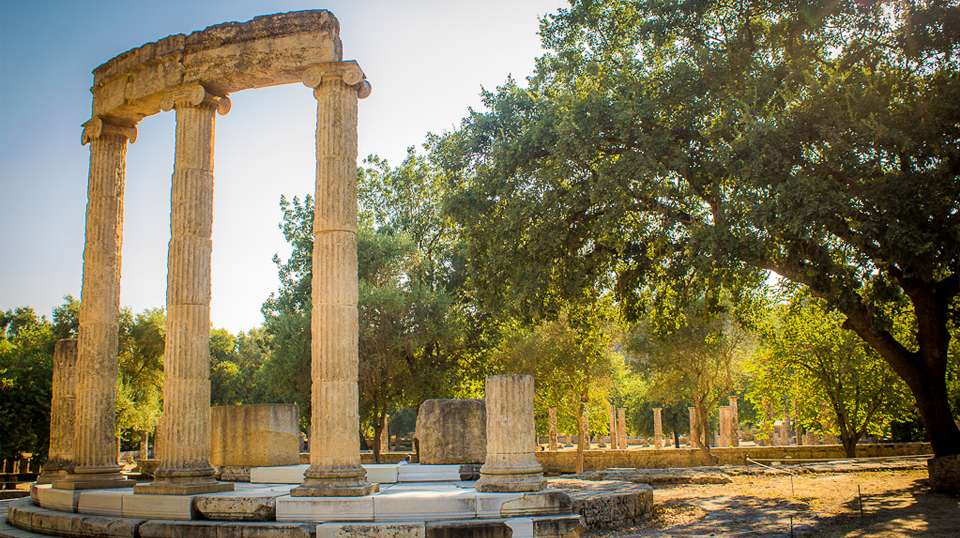
\includegraphics[width=55mm]{
               resources/olympia.jpg}
         };

         \node[anchor=east, xshift=-52pt, yshift=45pt]               
         at (current page.east) {
            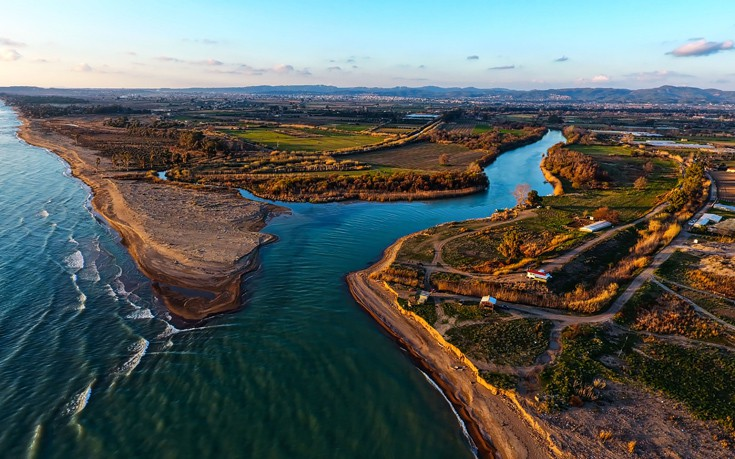
\includegraphics[width=55mm]{
               resources/alfios.jpg}
         };

      \end{tikzpicture}

      \begin{textblock*}{10cm}(1.0cm, 8.0cm)
         \small Great times with a lot of basketball and even more \textit{hows} and \textit{whys}
      \end{textblock*}

   \end{frame}

   % EKPA TIMES 
   \begin{frame}
      \frametitle{.. moves in Athens}
      \framesubtitle{Biology Department, National \& Kapodestrian University}
      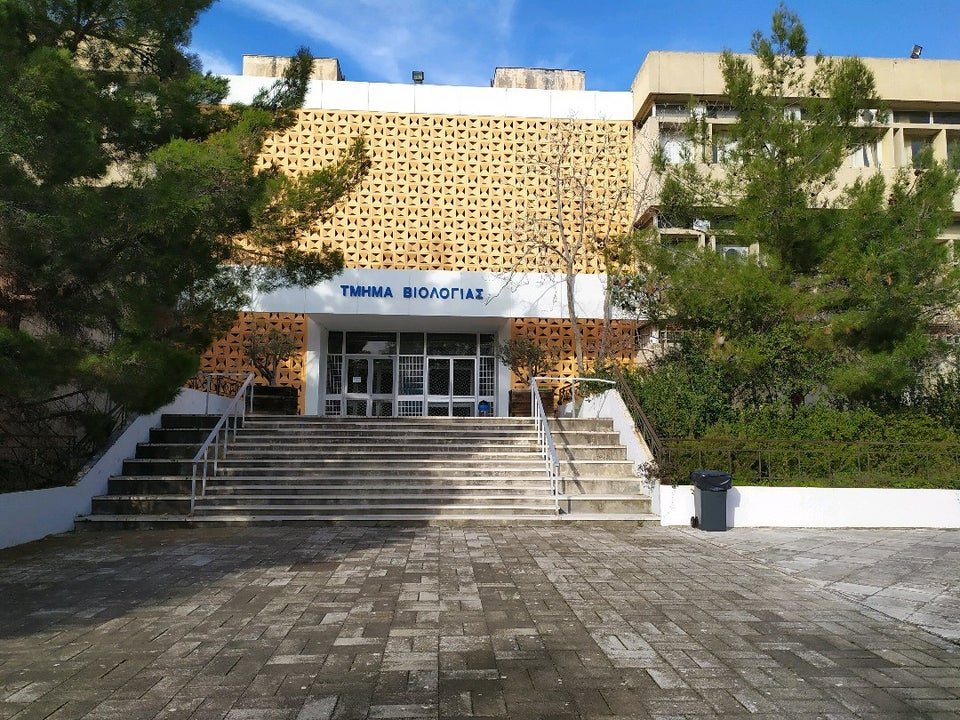
\includegraphics[width=60mm]{resources/biol_depart_ekpa.jpg} 
      \begin{textblock*}{5cm}(7.5cm, 5.0cm)
         \small Thesis on the morphology, morphometry and anatomy of species of the genus \textit{Pseudamnicola} in Greece
      \end{textblock*}
   \end{frame}

   % UoC TIMES 
   \begin{frame}

      \frametitle{.. and then to a "horrible" place called Crete}
      \framesubtitle{
         Medical School (MSc), Biology department (PhD) of UoC, \\
         Hellenic Centre for Marine Research
         }

      \begin{tikzpicture}

         \node[anchor=east, xshift=-130pt, yshift=30pt]               
         at (current page.east) {
            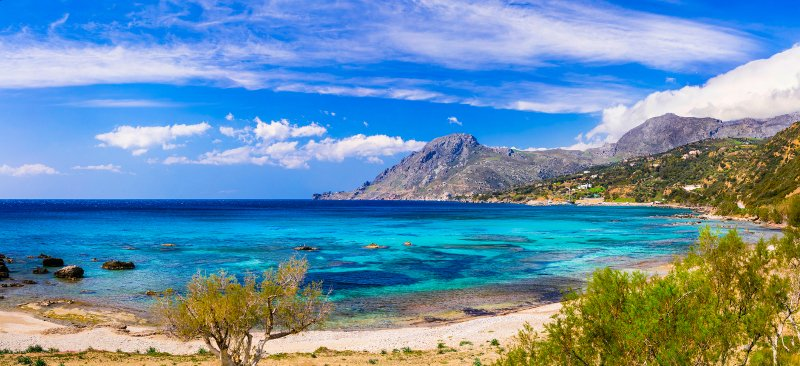
\includegraphics[width=60mm]{
               resources/plakias.jpg}
         };

         \node[anchor=east, 
         xshift=20pt]
         at (current page.east) {
            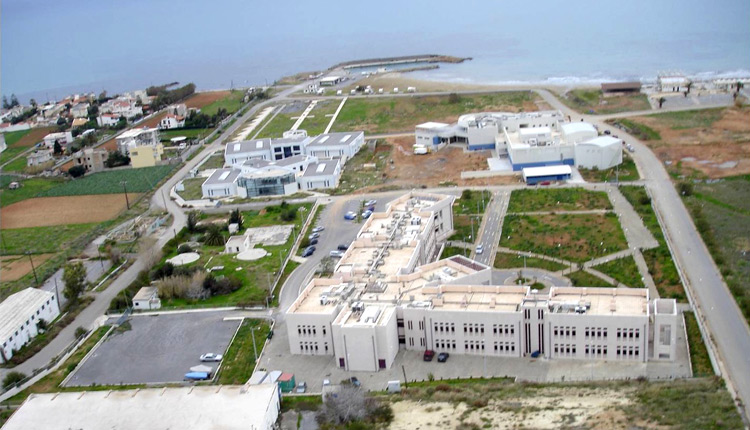
\includegraphics[width=50mm]{
               resources/hcmr.jpg}
         };

      \end{tikzpicture}

      % TEXT BLOCK
      \begin{textblock*}{10cm}(1.0cm, 8.0cm)

         \small MSc thesis on eDNA metabarcoding for biodiversity assessment: 
         Algorithm design and bioinformatics analysis pipeline implementation
         
      \end{textblock*}


   \end{frame}

   \fi
   % -------------------------------------- mute for the MARIKAT presentation ----------------------------


   % -------------------------
   % CHANGE THE CHAPTER SLIDE: MICROBIAL ECOLOGY INTRO
   % -------------------------
   \begin{darkframes}
      \section{
         Microbial ecology from a computational point-of-view
      }
   \end{darkframes}

   % INTRO
   \begin{frame}

      \frametitle{Microbial ecology \& biogeochemical cycles}
      \framesubtitle{a corner-stone for life on earth}

      \begin{figure}
         \centering
         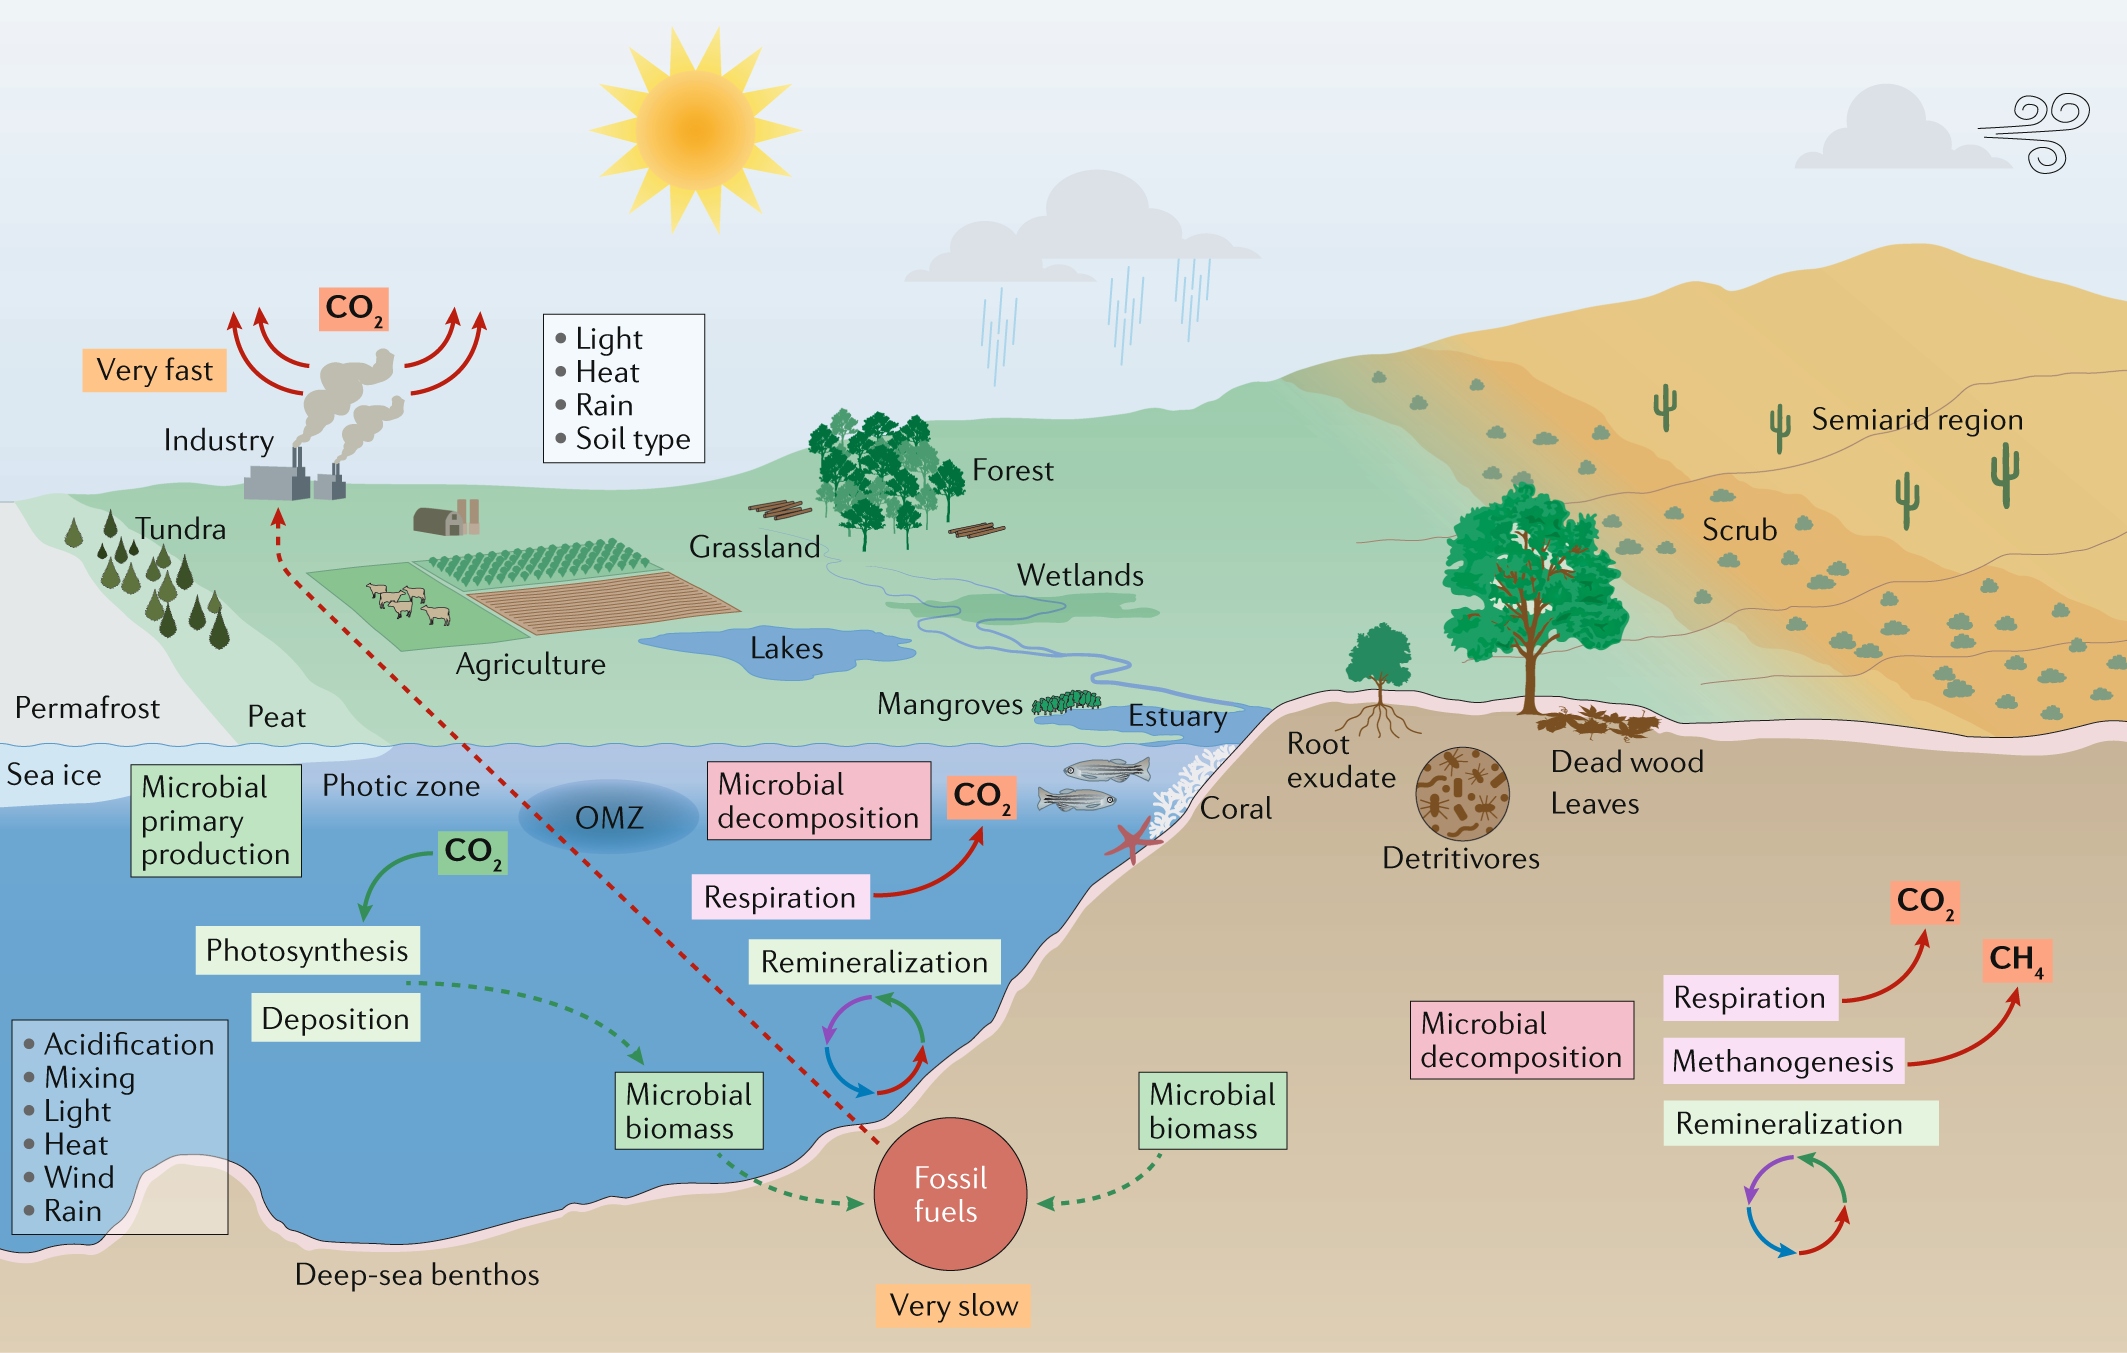
\includegraphics[width=85mm]{resources/ecosystem_functioning.png}
         \caption{
            \scriptsize Figure from: Cavicchioli et al.
            \scriptsize Nature Reviews Microbiology 17.9 (2019): 569-586.
         }
      \end{figure}
   \end{frame}

   % MAIN QUESTIONS 
   \begin{frame}
      \frametitle{Questions to address}
      \framesubtitle{for a deeper understanding of microbial assemblages}
      \begin{singlespace}


         \begin{columns}[onlytextwidth]
            
            \column{.33\textwidth}

               \begin{center}

                  Community \\ structure   \\ \textbf{\textit{who}}  

                  \hrulefill

                  \scriptsize \textit{eveyrone is everywhere}

               \end{center}


            \column{.33\textwidth}

               \begin{center}

                  Functional \\ potential \\ \textbf{\textit{what}}

                  \hrulefill

                  \scriptsize \textit{zero-sum game}

               \end{center}

            \column{.33\textwidth}

               \begin{center}

                  Microbial \\ interactions \\ \textbf{\textit{why / how}}

                  \hrulefill

                  \scriptsize \textit{the entagnled bank}

               \end{center}
      

         \end{columns}

      \end{singlespace}

   \end{frame}

   % BIOINFORMATICS 
   \begin{frame}

      \frametitle{We are living in a computational era}
      \framesubtitle{both a challenge \& an opportunity}
      \centering
      
\includegraphics[width=85mm]{resources/bioinfo_transparent.png}

   \end{frame}



   % % -------------------------
   % % CHANGE THE CHAPTER SLIDE: HIGH THROUGHPUT SEQUENCING INTRO
   % % -------------------------

   % \begin{darkframes}
   %    \section{
   %       Bioinformatics methods for microbial diversity assessment
   %    }
   
   % \end{darkframes}

   % % MARKER GENES - BIOINFO STEPS
   % \begin{frame}
      
   %    \frametitle{eDNA metabarcoding}
   %    \framesubtitle{for biodiversity assessment}
   %    \begin{singlespace}


   %       \begin{columns}[onlytextwidth]

   %          \column{.5\textwidth}

   %             \textbf{Marker genes} \\ 

   %             \begin{enumerate}
   %                \item \textbf{16S rRNA:} Bacteria, Archaea
   %                \item \textbf{12S rRNA:} Vertebrates
   %                \item \textbf{18S rRNA:} Small eukaryotes, Metazoa
   %                \item \textbf{ITS:} Fungi
   %                \item \textbf{COI:} Eukaryotes
   %                \item \textbf{\textit{rbcl}:} Plants
   %                \item \textbf{\textit{dsrb}:} Bacteria, Archaea
   %                \item ...
   %             \end{enumerate}

   %          \column{.45\textwidth}

   %             \textbf{Methodology}

   %             \begin{figure}
   %                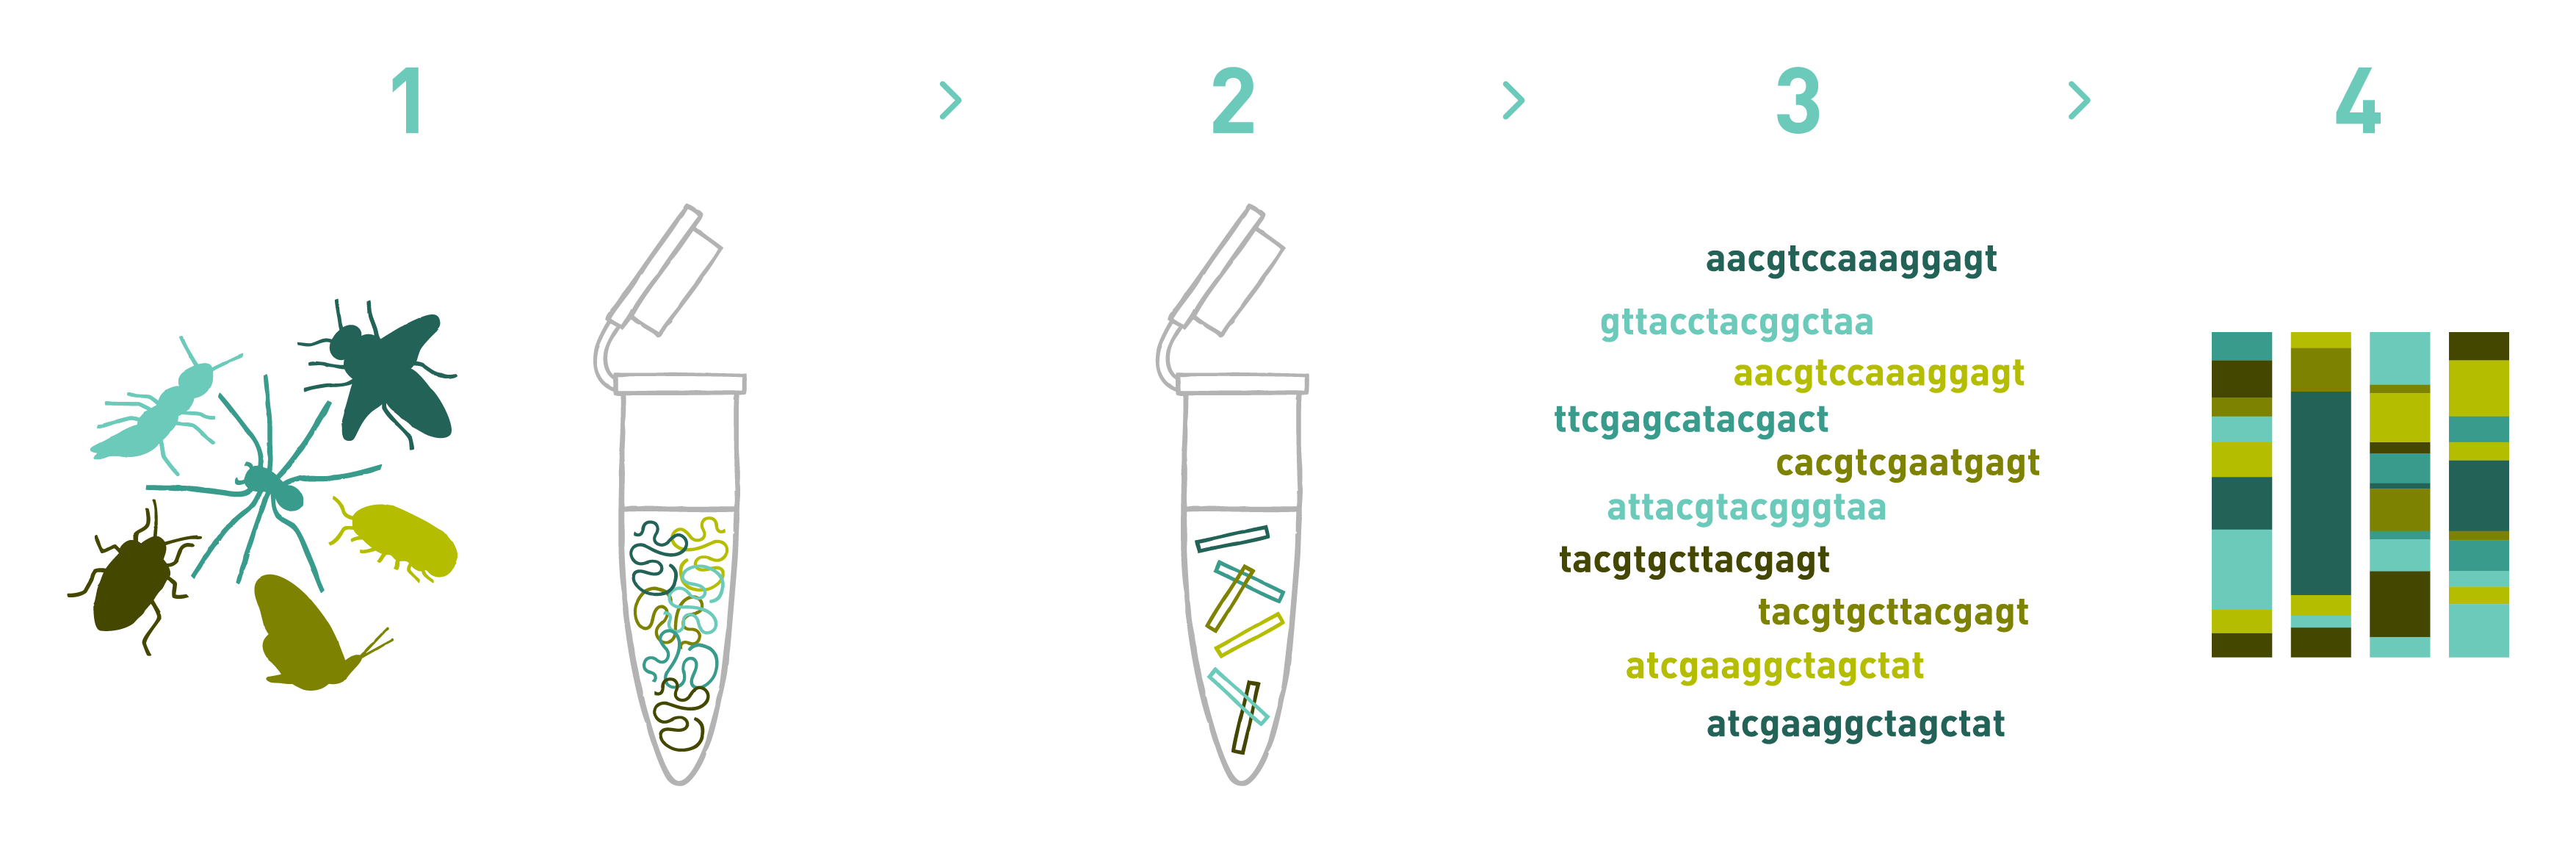
\includegraphics[width=55mm]{resources/metabarcoding-steps.png}
   %             \end{figure}

   %             \begin{itemize}
   %                \item Sampling
   %                \item Extraction
   %                \item Bioinformatics
   %                \item Biodiversity analysis
   %             \end{itemize}
               

   %       \end{columns}

   %    \end{singlespace}
   % \end{frame}

   % % BIOINFORMATICS CHALLENGES 
   % \begin{frame}
   %    \frametitle{Bioinformatics challenges}
   %    \framesubtitle{for the analysis and the interpretation of amplicon data}

   %    \begin{columns}[onlytextwidth]

   %       \column{.5\textwidth}

   %          
\includegraphics[width=40mm]{resources/bioinfo_mess.png}

   %       \column{.5\textwidth}

   %          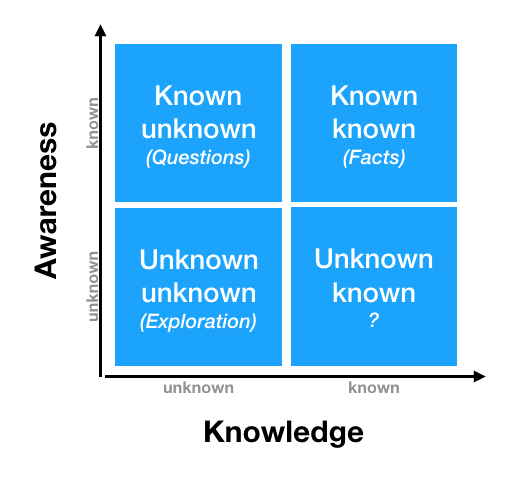
\includegraphics[width=50mm]{resources/known_unknown.png}
         
   %    \end{columns}
   % \end{frame}


   % -------------------------
   % CHANGE SUBSECTION: PEMA 
   % -------------------------

   % BRIDGE SLIDE
   \begin{darkframes}

      \section{\texttt{PEMA}: a metabarcoding pipeline}

      % PEMA LOGO
      \begin{frame}

         \begin{figure}
            \centering
            
\includegraphics[width=60mm]{resources/pema_logo.png}         
         \end{figure} 

         \begin{textblock*}{7cm}(3.1cm, 8.2cm)
            \centering
            \href{https://github.com/hariszaf/pema}{https://github.com/hariszaf/pema} \\ 
            \href{http://pema.hcmr.gr}{pema.hcmr.gr}
         \end{textblock*}


      \end{frame}

   \end{darkframes}


   % MARKER GENES - BIOINFO STEPS
   \begin{frame}
      
      \frametitle{eDNA metabarcoding}
      \framesubtitle{for biodiversity assessment}
      \begin{singlespace}


         \begin{columns}[onlytextwidth]

            \column{.5\textwidth}

               \textbf{Marker genes} \\ 

               \begin{enumerate}
                  \item \textbf{16S rRNA:} Bacteria, Archaea
                  \item \textbf{12S rRNA:} Vertebrates
                  \item \textbf{18S rRNA:} Small eukaryotes, Metazoa
                  \item \textbf{ITS:} Fungi
                  \item \textbf{COI:} Eukaryotes
                  \item \textbf{\textit{rbcl}:} Plants
                  \item \textbf{\textit{dsrb}:} Bacteria, Archaea
                  \item ...
               \end{enumerate}

            \column{.45\textwidth}

               \textbf{Methodology}

               \begin{figure}
                  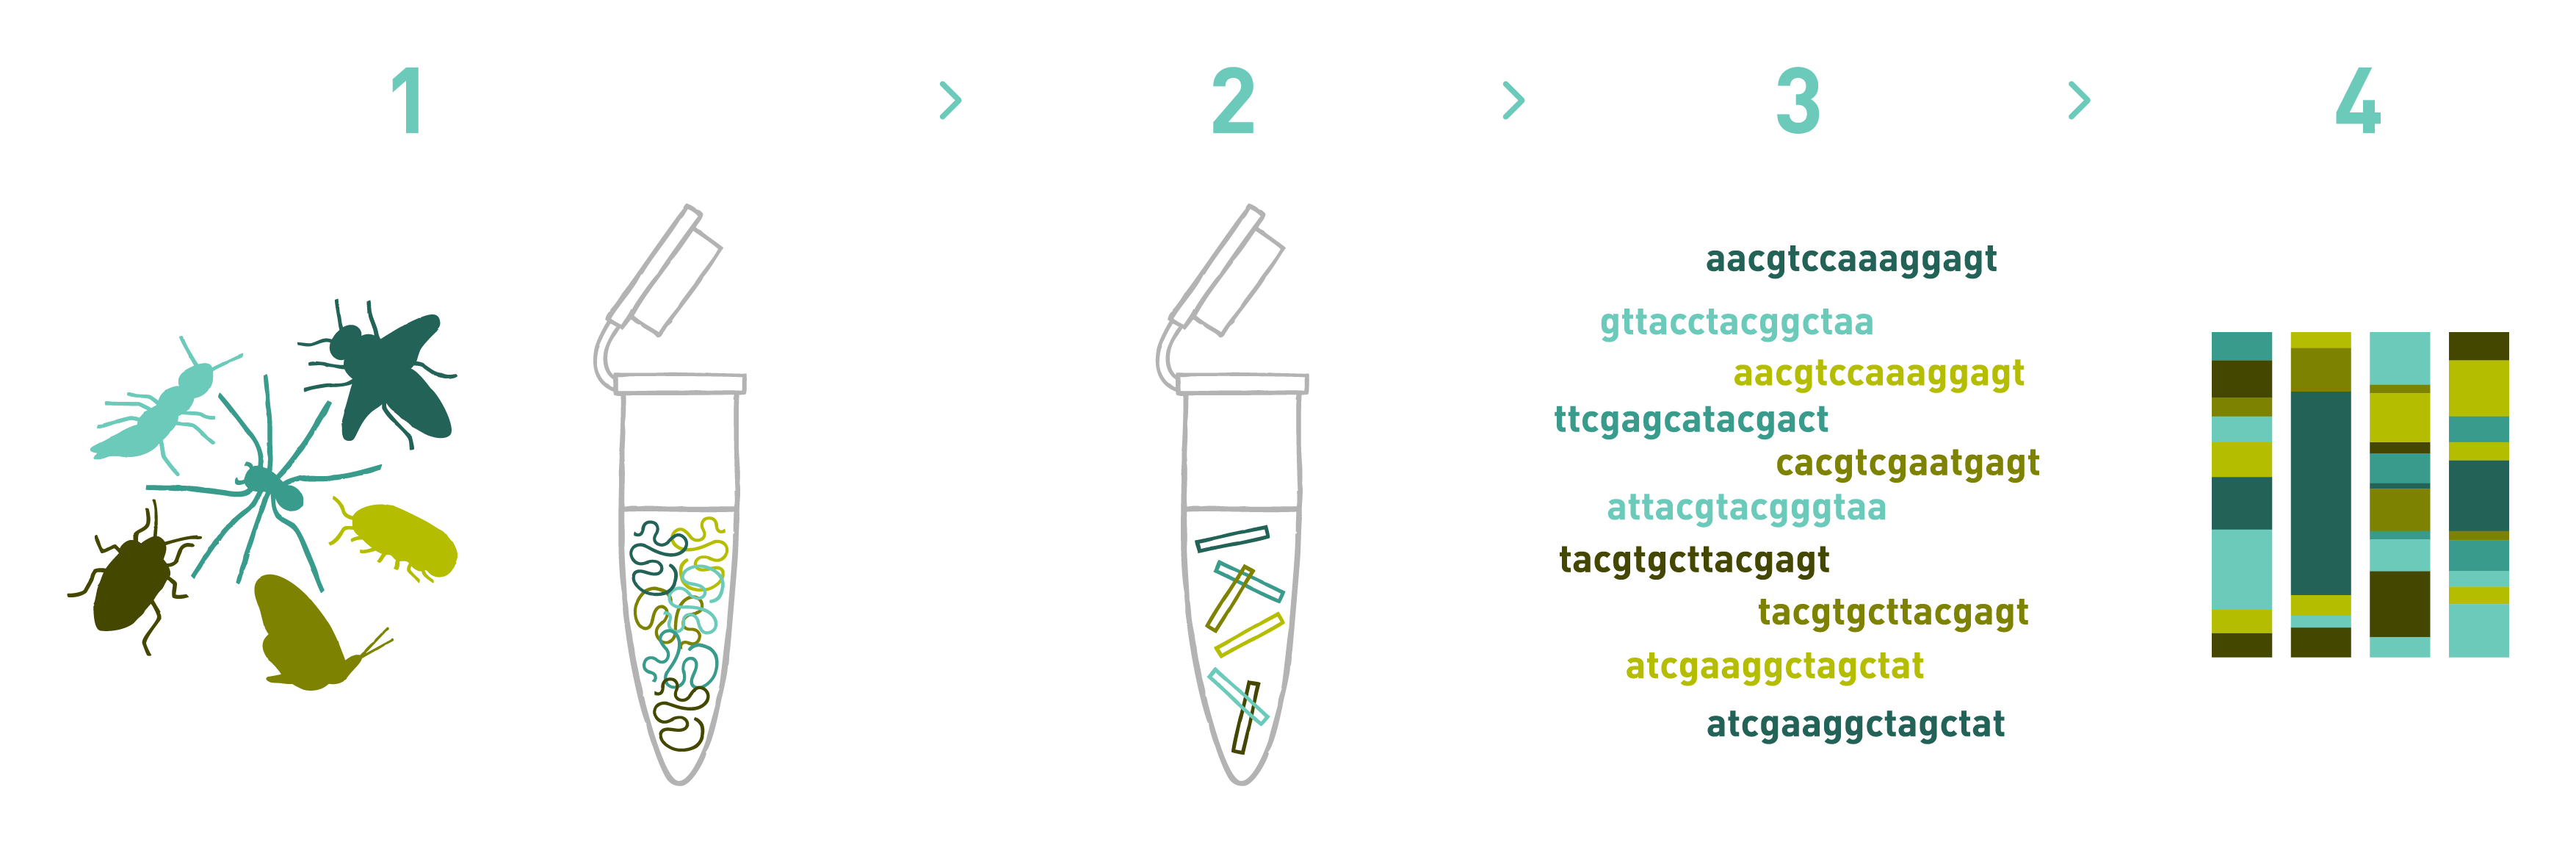
\includegraphics[width=55mm]{resources/metabarcoding-steps.png}
               \end{figure}

               \begin{itemize}
                  \item Sampling
                  \item Extraction
                  \item Bioinformatics
                  \item Biodiversity analysis
               \end{itemize}
               

         \end{columns}

      \end{singlespace}
   \end{frame}


   % WORKFLOW SLIDE
   \begin{frame}
      \frametitle{PEMA features}
      \framesubtitle{one step at a time!}
      \begin{singlespace}
         \begin{tikzpicture}[overlay,remember picture]
            \node[anchor=west, xshift=30pt,yshift=-165pt]
               at (current page.north west) {
                  \includegraphics[width=104mm]{resources/pema-pema.drawio.png}
               };

         \end{tikzpicture}
      \end{singlespace}
   \end{frame}

   % PHYLOGENY TREE
   \begin{frame}
      \frametitle{PEMA features}
      \framesubtitle{one step at a time!}
      \begin{singlespace}
         \begin{tikzpicture}[overlay,remember picture]
            \node[anchor=west, xshift=30pt,yshift=-165pt]
               at (current page.north west) {
                  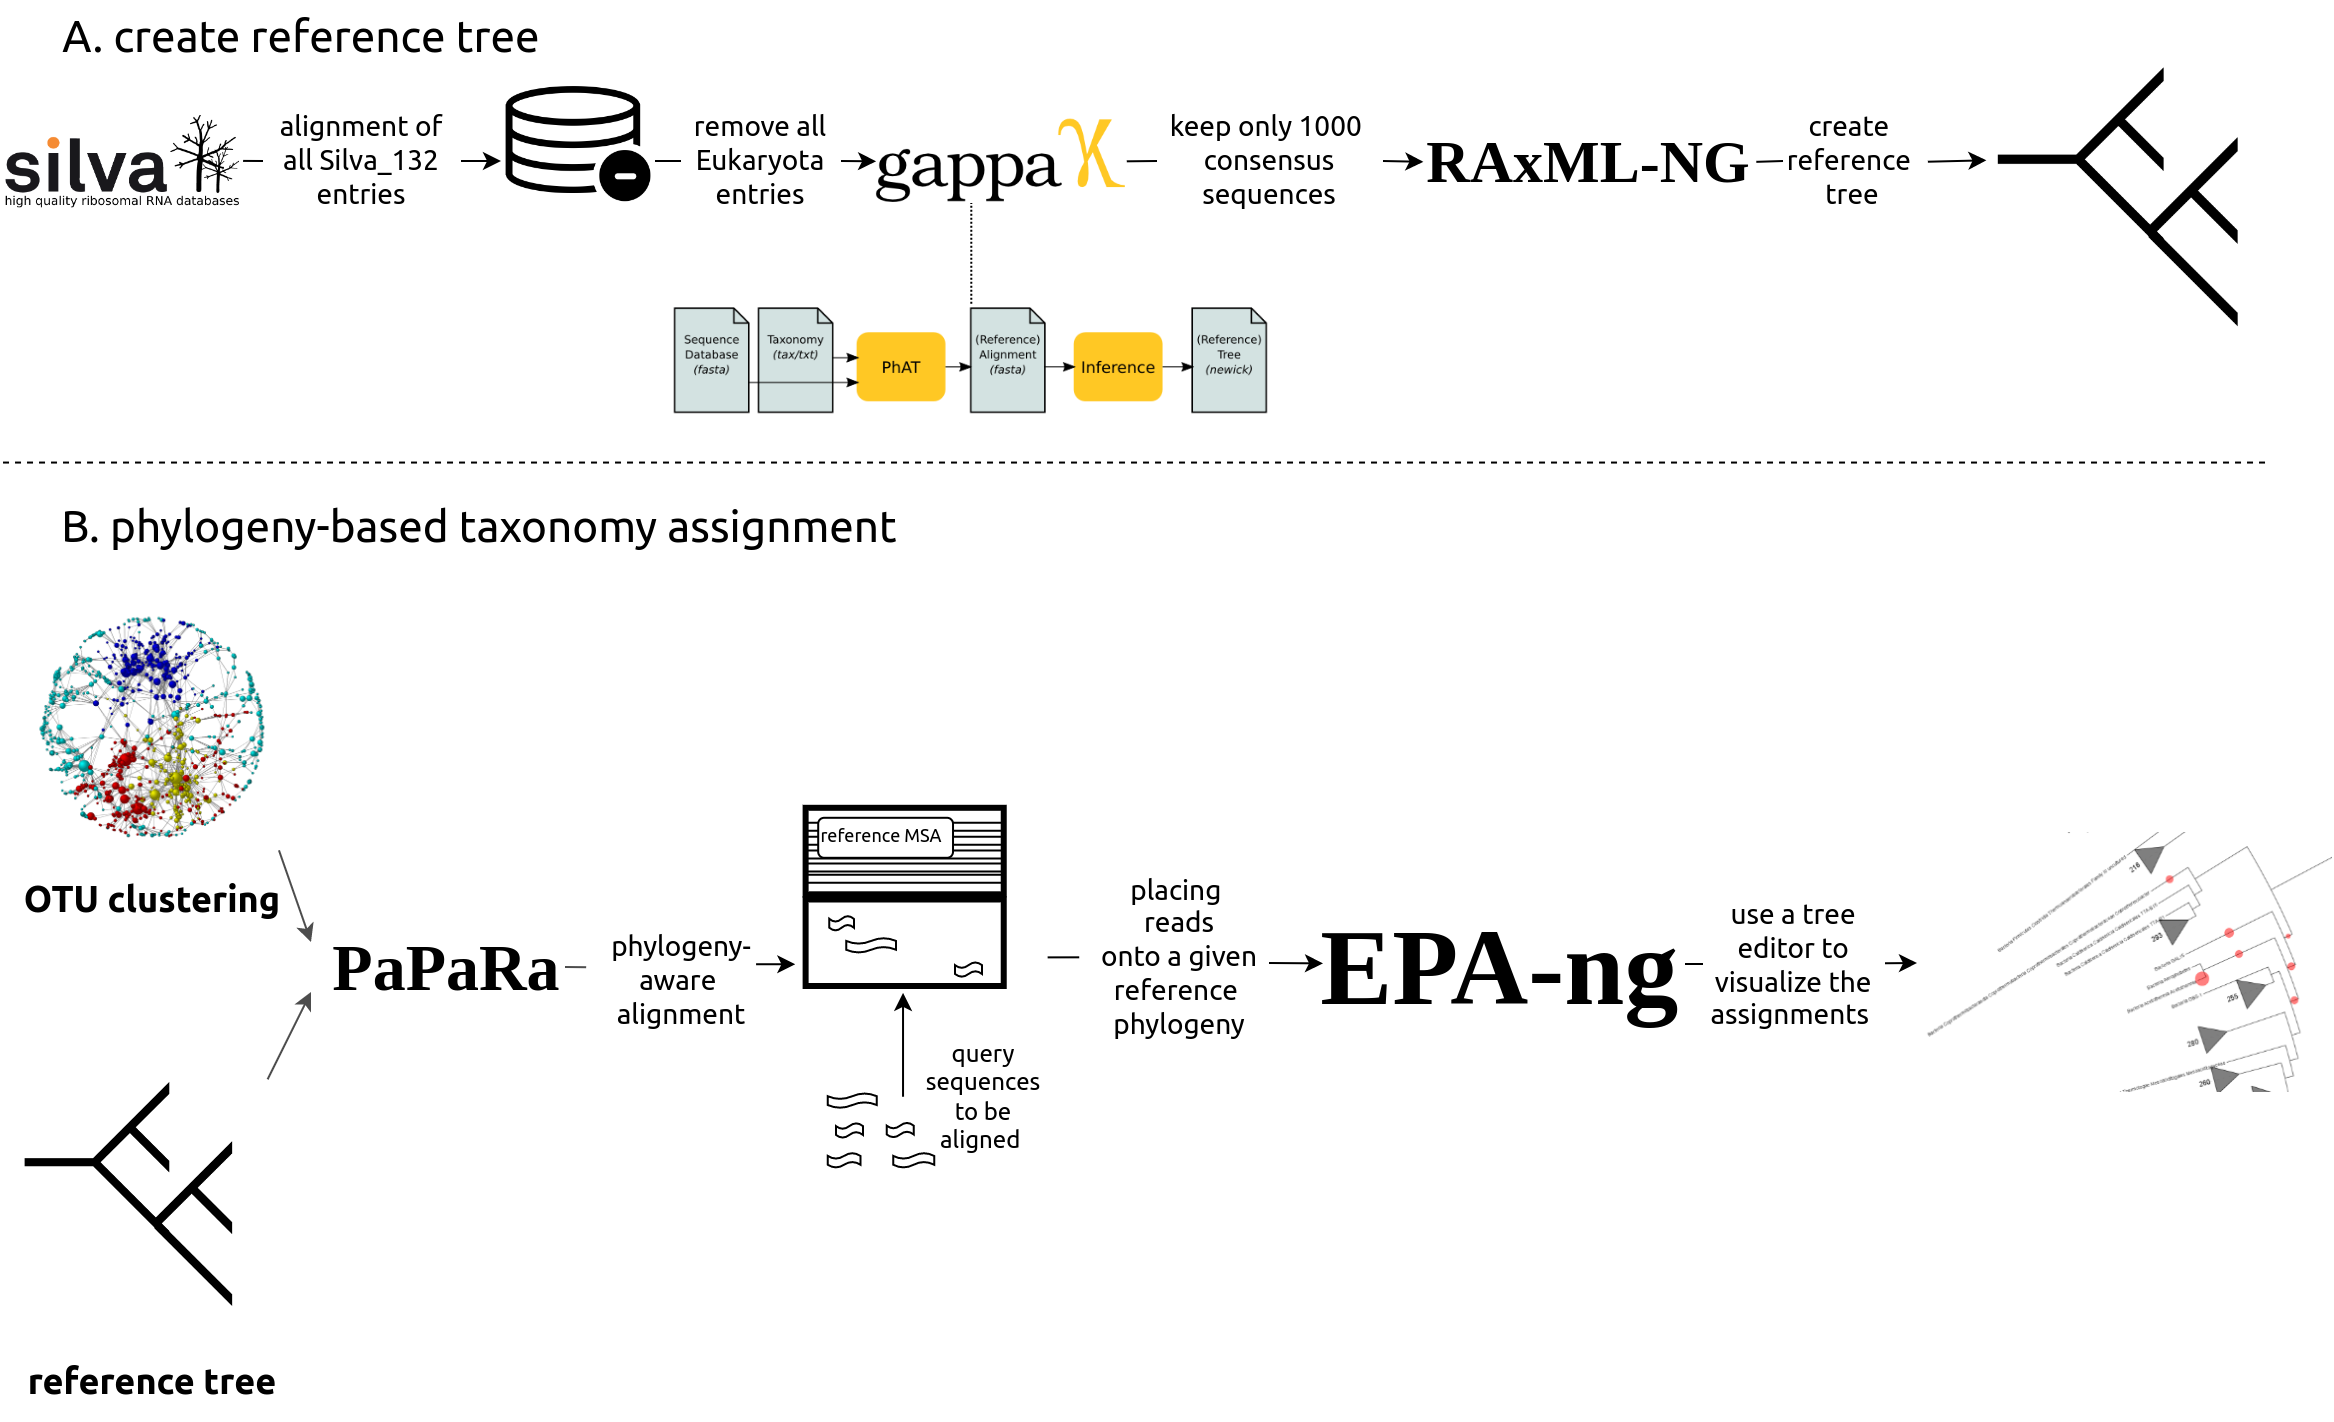
\includegraphics[width=104mm]{resources/pema_tree.png}
               };

         \end{tikzpicture}
      \end{singlespace}
   \end{frame}

   % BIOINFORMATICS TRICKS AND HINTS
   \begin{frame}
      \frametitle{PEMA coding insights}
      \framesubtitle{Being a \texttt{geek} just for a bit !}

      \begin{columns}[onlytextwidth]
         
         \column{0.5\textwidth}
         
            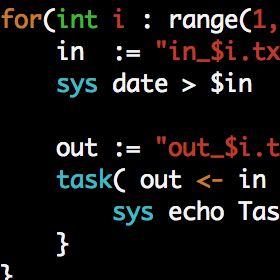
\includegraphics[width=25mm]{resources/bds.png}

            \texttt{BigDataScript} \\
            programming language

         \column{0.5\textwidth}

            \begin{tikzpicture}[overlay,remember picture]

               \node[anchor=east, xshift=-130pt, yshift=10pt]               
                  at (current page.east) {

                     
\includegraphics[width=20mm]{resources/sing_transp.png}
                  
                  };

                  \node[anchor=east, xshift=-40pt, yshift=10pt]
                  at (current page.east) {

                     
\includegraphics[width=25mm]{resources/docker_facebook_share.png}
                  
                  };

                  \node[anchor=south, align = center, above, xshift=60, yshift=90]
                  at (current page.south) {

                     Containerization

                  };

            \end{tikzpicture}
            
            % \bigskip
            % Containerization


      \end{columns}


   \end{frame}

   % INPUT - OUTPUT - RUN WITH A SINGLE COMMAND
   \begin{frame}

      \frametitle{Mount your I/O}
      \framesubtitle{give \& take}

      \begin{tikzpicture}[overlay,remember picture]

         \node[anchor=west, xshift=10pt, yshift=-10pt]               
            at (current page.west) {

               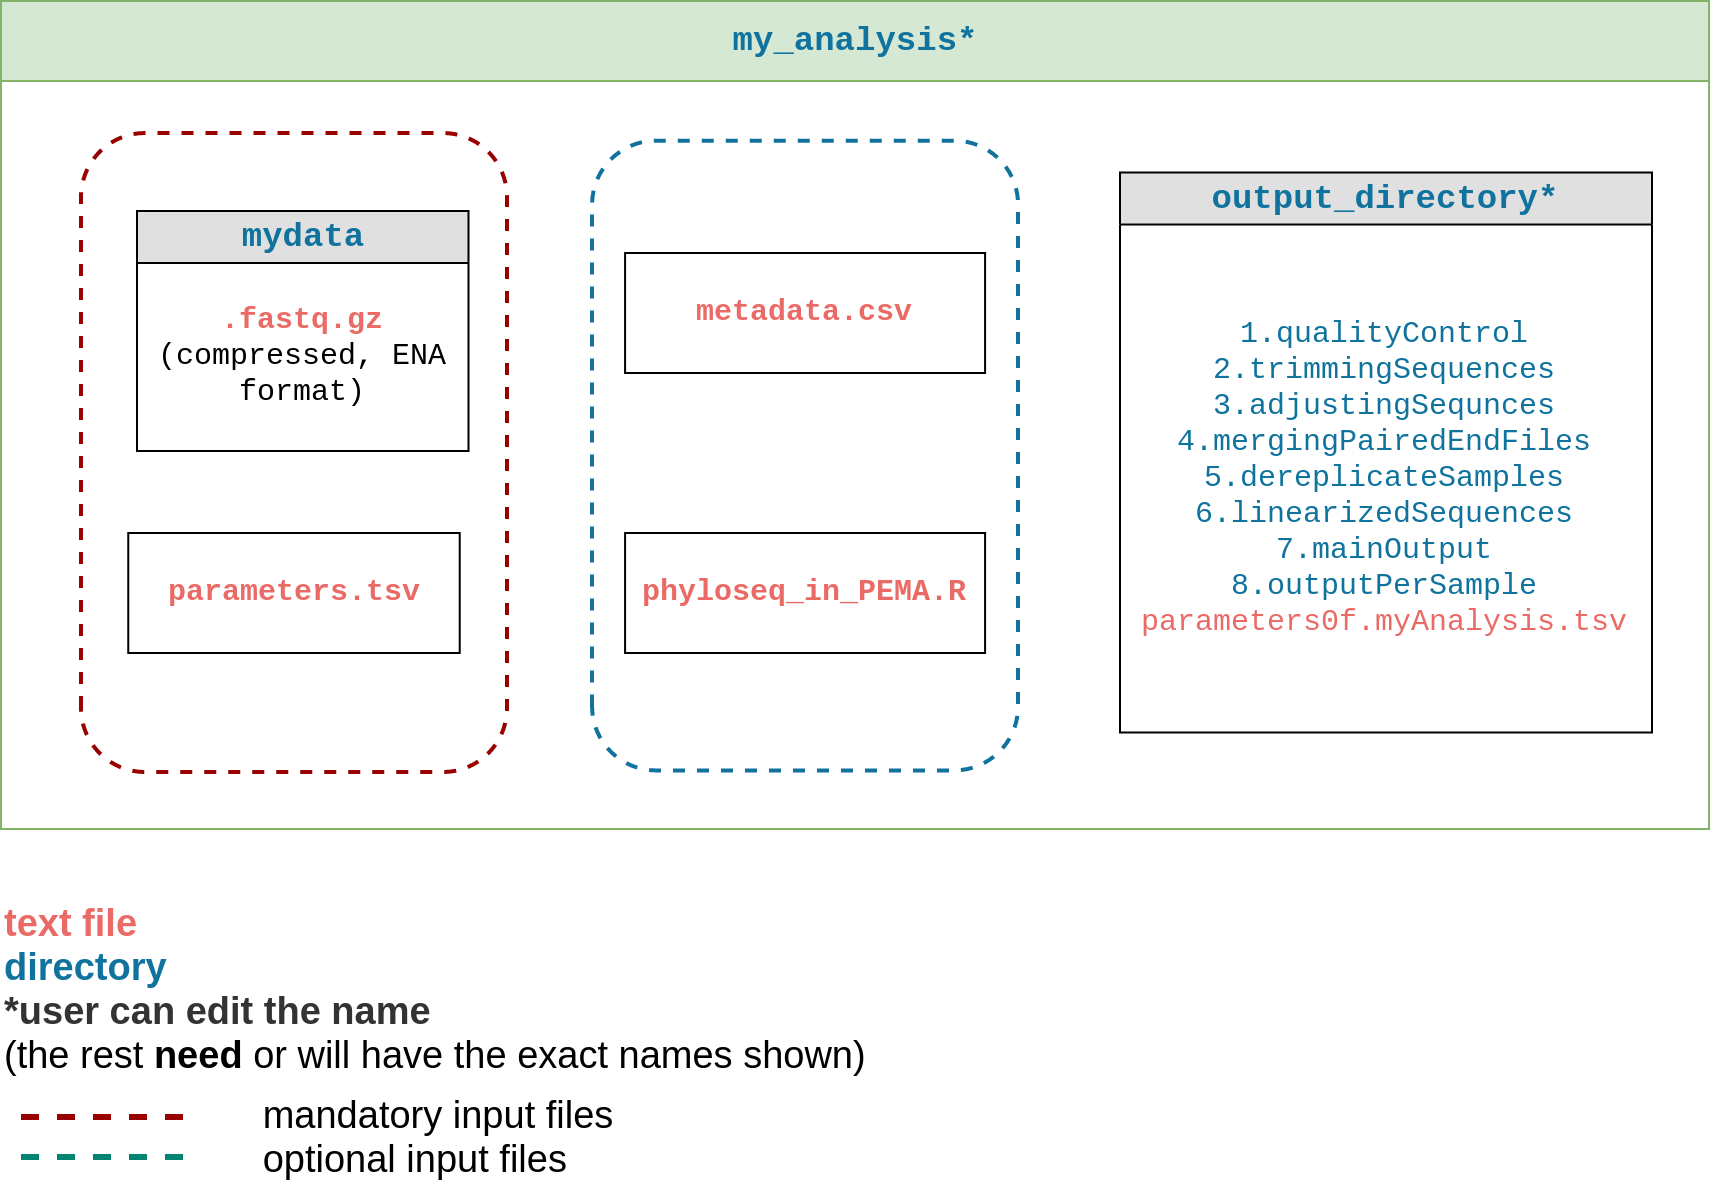
\includegraphics[width=75mm]{resources/pema_anlysis_dir-Page-1.drawio.png}
            
            };

         \node[anchor=east, xshift=-10pt, yshift=50pt]               
         at (current page.east) {

            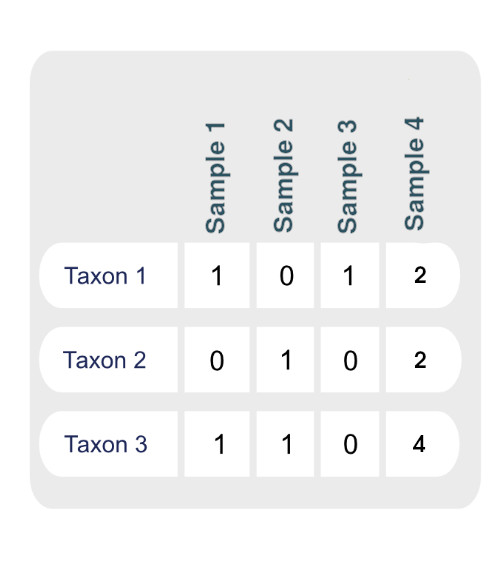
\includegraphics[width=35mm]{resources/final_table.jpg}
         
         };

         \node[anchor=east, xshift=-10pt, yshift=-60pt]
         at (current page.east) {

            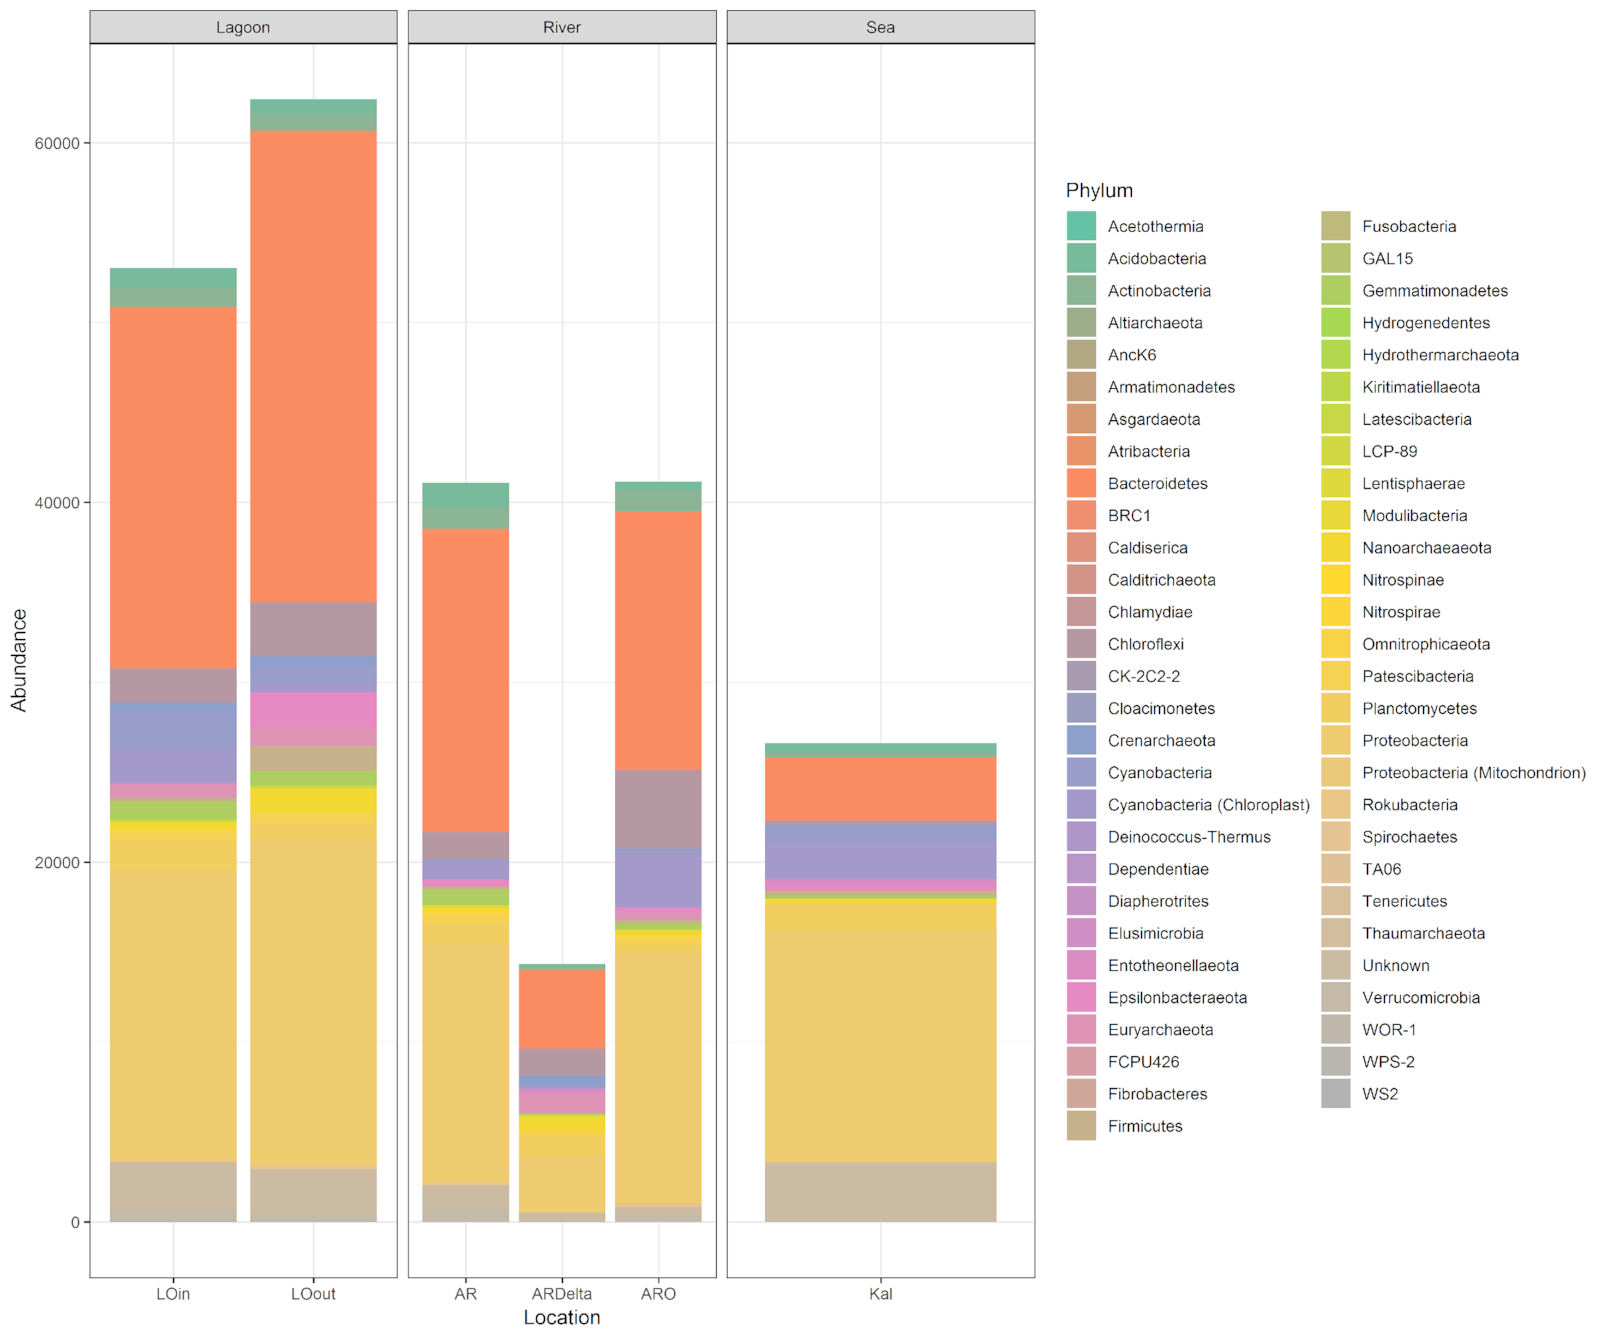
\includegraphics[width=43mm]{resources/giaa022fig3.jpeg}
         
         };


      \end{tikzpicture}
      
   
   \end{frame}

   % % PEMA PUBLICATION 
   % \begin{frame}
   %    \frametitle{PEMA publication}
   %    \framesubtitle{in 2020}
   %    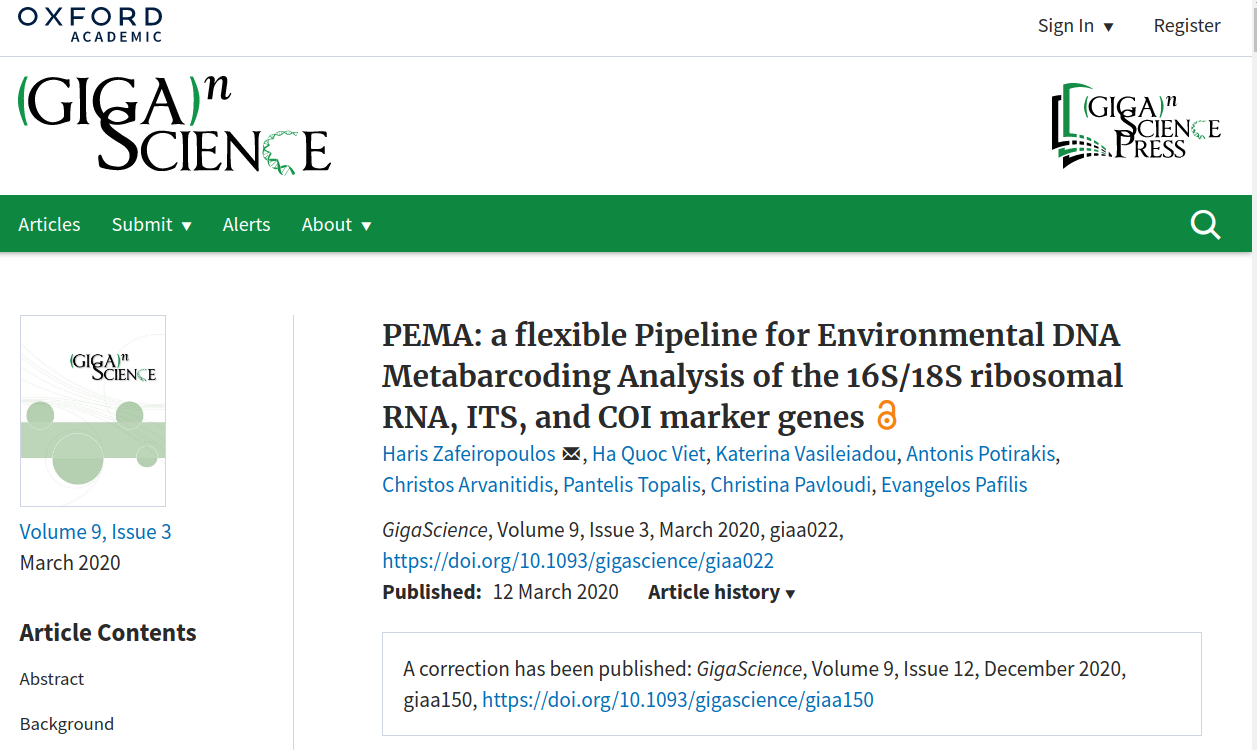
\includegraphics[width=100mm]{resources/pema_publ.png}
   % \end{frame}

   % PEMA VERSION 2
   \begin{frame}
      \frametitle{PEMA v.2}
      \framesubtitle{addressing some of the challenges}

      \begin{singlespace}
         \begin{tikzpicture}[overlay,remember picture]
       
               \node[anchor=west, xshift=30pt,yshift=-150pt]
                  at (current page.north west) {
                     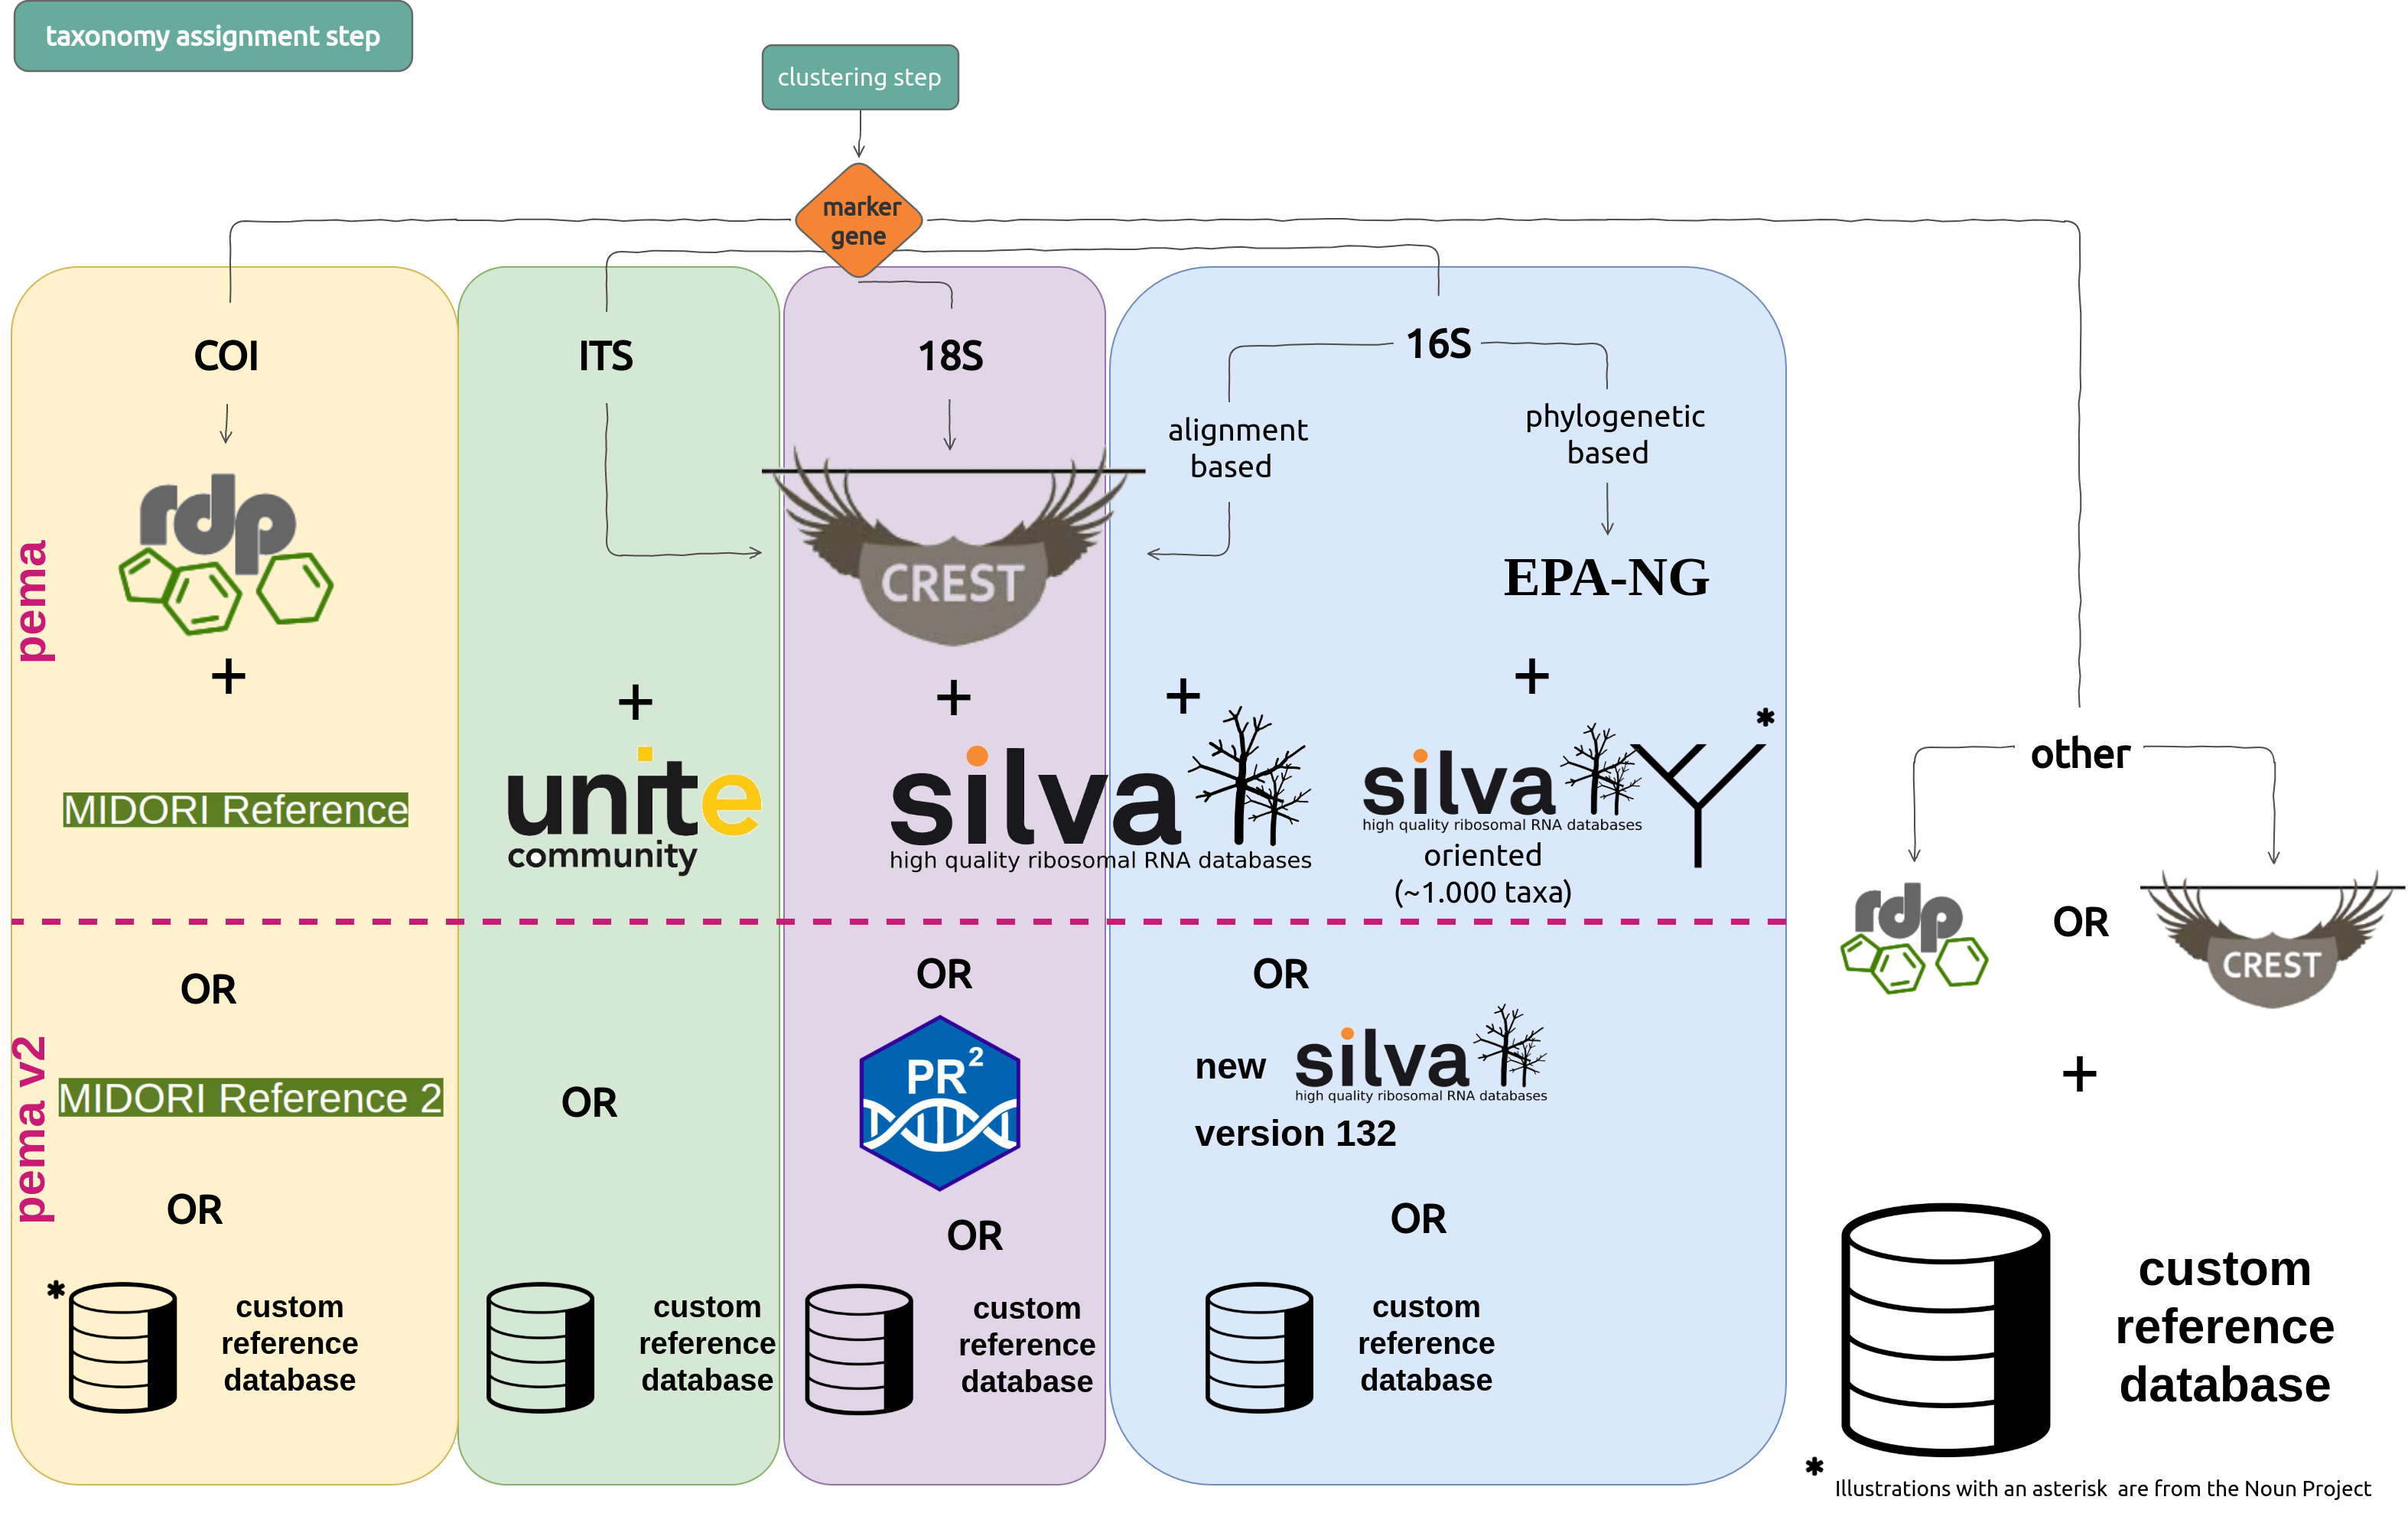
\includegraphics[width=100mm]{resources/pema-pema.v2.drawio.png}
                  };
                  
         \end{tikzpicture}

         \begin{textblock*}{5cm}(8.2cm, 2.3cm) % {block width} (coords) 
            
            \scriptsize Code architecture from scratch!

         \end{textblock*}

      \end{singlespace}
   \end{frame}

   % PEMA v.2.1.4 - ARMS
   \begin{frame}
      \frametitle{Latest PEMA version}
      \framesubtitle{addressing the challenges of the community}

      \begin{singlespace}
         \begin{tikzpicture}[overlay,remember picture]
       
               \node[anchor=west, xshift=30pt,yshift=-150pt]
                  at (current page.north west) {
                     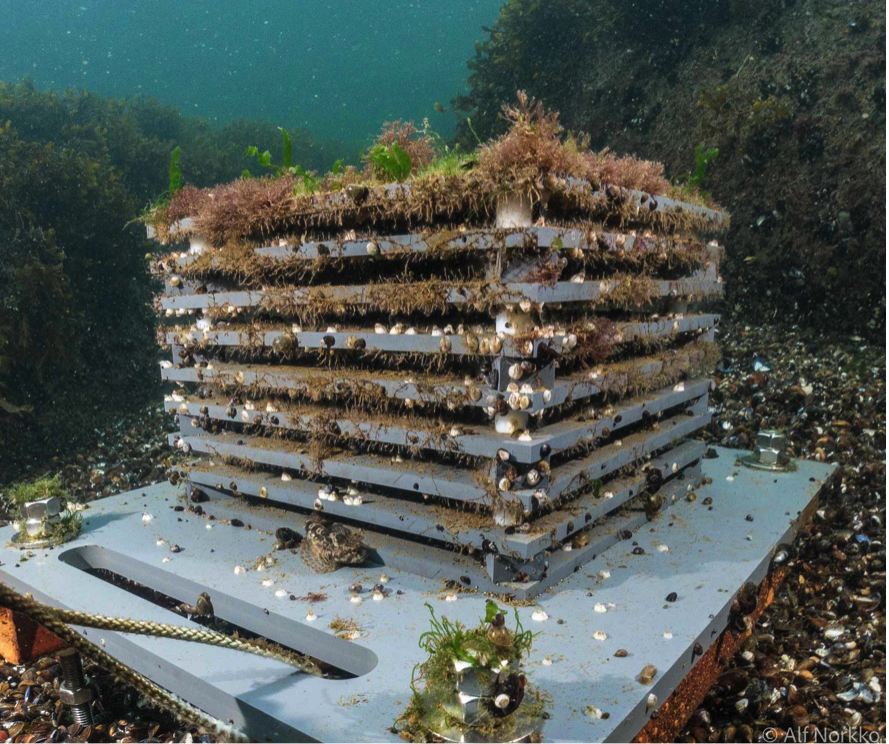
\includegraphics[width=55mm]{resources/Autonomous-Reef-Monitoring.png}
               };

               \node[anchor=east, xshift=-65pt,yshift=50pt]
                  at (current page.east) {
                     
\includegraphics[width=34mm]{resources/assemble_logo.png}
               };

               \node[anchor=east, xshift=-5pt,yshift=50pt]
                  at (current page.east) {
                     
\includegraphics[width=17mm]{resources/MBON_logo_transparent.png}

               };

         \end{tikzpicture}


         \begin{textblock*}{5cm}(7.2cm,4.0cm) % {block width} (coords) 
            
            \scriptsize

            \textbf{\texttt{pema:v.2.1.4} includes:}

            \begin{enumerate}
               \item analysis of 12S rRNA data now supported
                     (\href{https://github.com/terrimporter/12SvertebrateClassifier/releases}{12S Vertebrate Classifier v2.0.0-ref} database) 
               \item PR2 as an alternative reference 
                     database for the case of 18S rRNA 
               \item the \texttt{ncbi-taxonomist} tool \\ 
                     was added to return the NCBI Taxonomy \\ 
                     Id of the taxonomies found
            \end{enumerate}

         \end{textblock*}


      \end{singlespace}
   \end{frame}

   % GitHub repo -- the pema_contribution picture is missing
   \if 0
   \begin{frame}
   \frametitle{open source is cool}
      \framesubtitle{interacting with the community}

      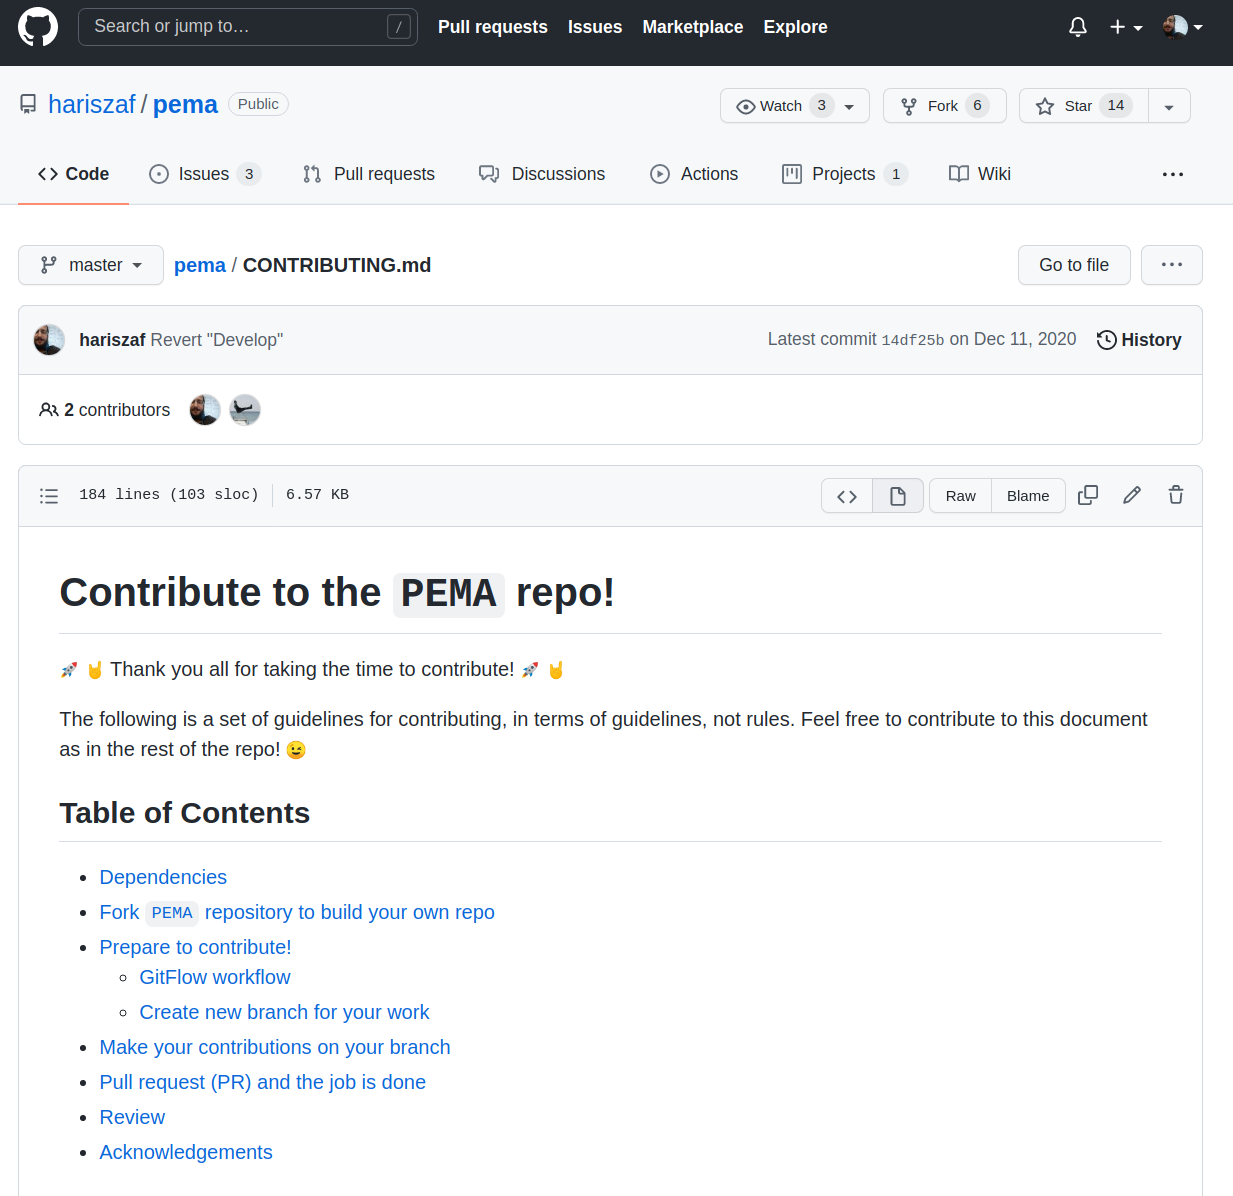
\includegraphics[width=60mm]{resources/pema_contribution.png}

      \small
      \begin{textblock*}{5cm}(7.5cm,4.0cm) % {block width} (coords) 
         PEMA aims at building a community 
         to discuss challenges on metabarcoding
         come up with solutions and why not 
         develop some of them! 
      \end{textblock*}

   \end{frame}
   \fi

   % PEMA WEBSITE
   \begin{frame}
      \frametitle{\textit{How to} and further documentation}
      \framesubtitle{at \href{http://pema.hcmr.gr}{pema.hcmr.gr}}
      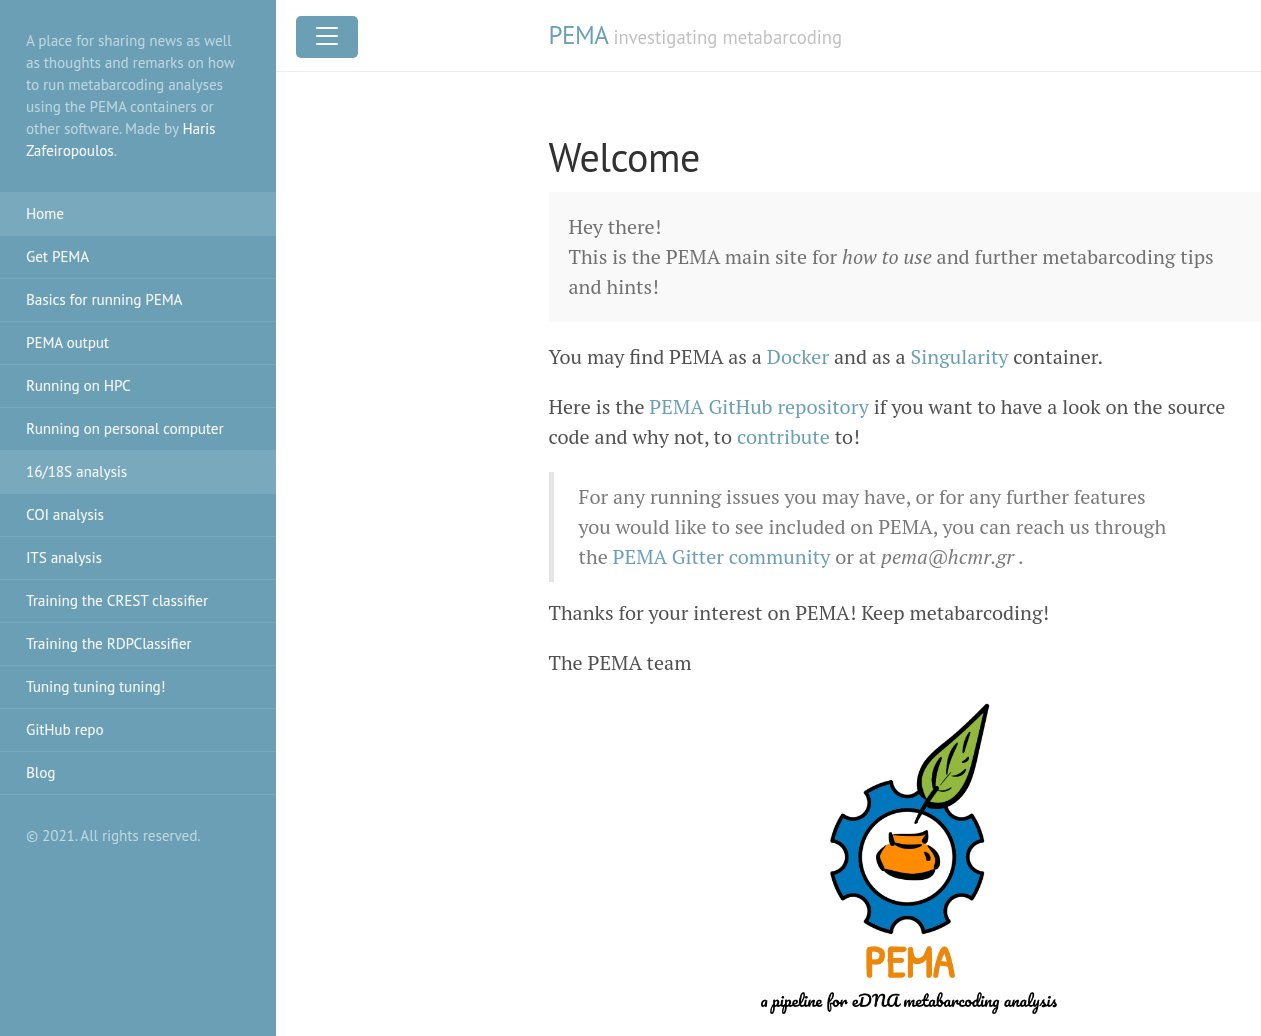
\includegraphics[width=85mm]{resources/pema_site.png}
   \end{frame}


   % EOSC Life GOs
   \begin{frame}
      \frametitle{Metagenome go deeper than amplicon studies}
      \framesubtitle{yet come with vast computational challenges}
      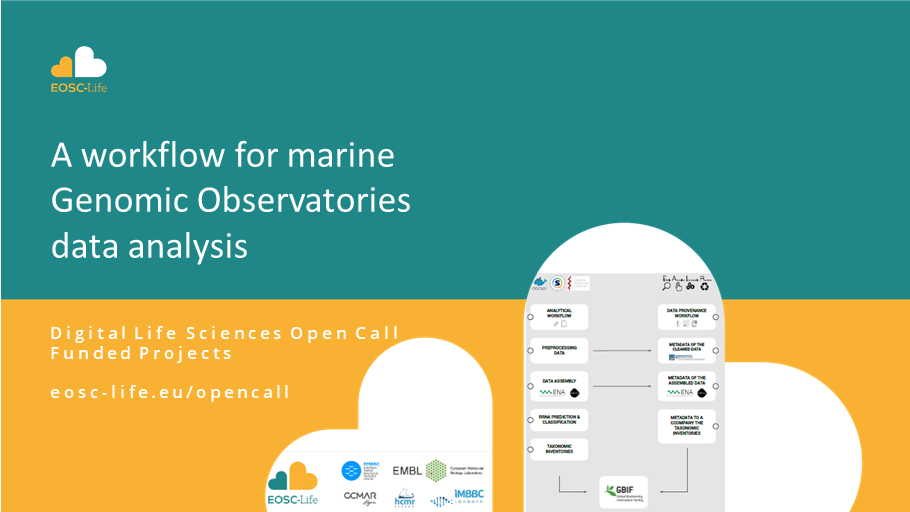
\includegraphics[width=70mm]{resources/marine-genomic-observatories.png}

      \begin{textblock*}{5cm}(8.5cm,4.0cm) % {block width} (coords) 
            
         \textbf{Work in progress} \\
         To be available in the \\ months to come.

         \bigskip
         
         \footnotesize
         You may find more \\ 
         \footnotesize
         about this project  \\
         \footnotesize
         through its \href{https://github.com/emo-bon/pipeline-v5}{GitHub repository}

      \end{textblock*}


   \end{frame}


   % % -------------------------------------
   % % CHANGE SUBSECTION: DARN
   % % -------------------------------------

   % % DARN LOGO SLIDE
   % \begin{darkframes}
   %    \subsection{\texttt{darn}: known unknowns in COI amplicon data}
   %    \begin{frame}
   %       \begin{figure}
   %          
\includegraphics[width=55mm]{resources/darn_logo.png}
   %          
\includegraphics[width=30mm]{../met_nets/resources/darn-logo-text.png}
   %       \end{figure}


   %       \begin{textblock*}{7cm}(3.5cm, 7.0cm)
   %          \href{https://github.com/hariszaf/darn}{https://github.com/hariszaf/darn}
   %       \end{textblock*}


   %    \end{frame}
   % \end{darkframes}

   % % DARN METHODOLOGY
   % \begin{frame}
   %    \frametitle{Dark mAtteR iNvesigator}
   %    \framesubtitle{investigating known unknown \\ in COI amplicon data}

   %    \begin{textblock*}{7cm}(1.2cm, 4.5cm)
   %       What is all these unassigned  \\
   %       OTUs / ASVs? 
   %    \end{textblock*}

   %    \begin{singlespace}
   %       \begin{tikzpicture}[overlay,remember picture]
   %          \node[anchor=north east, xshift=-10pt,yshift=-5pt]
   %             at (current page.north east) {
   %                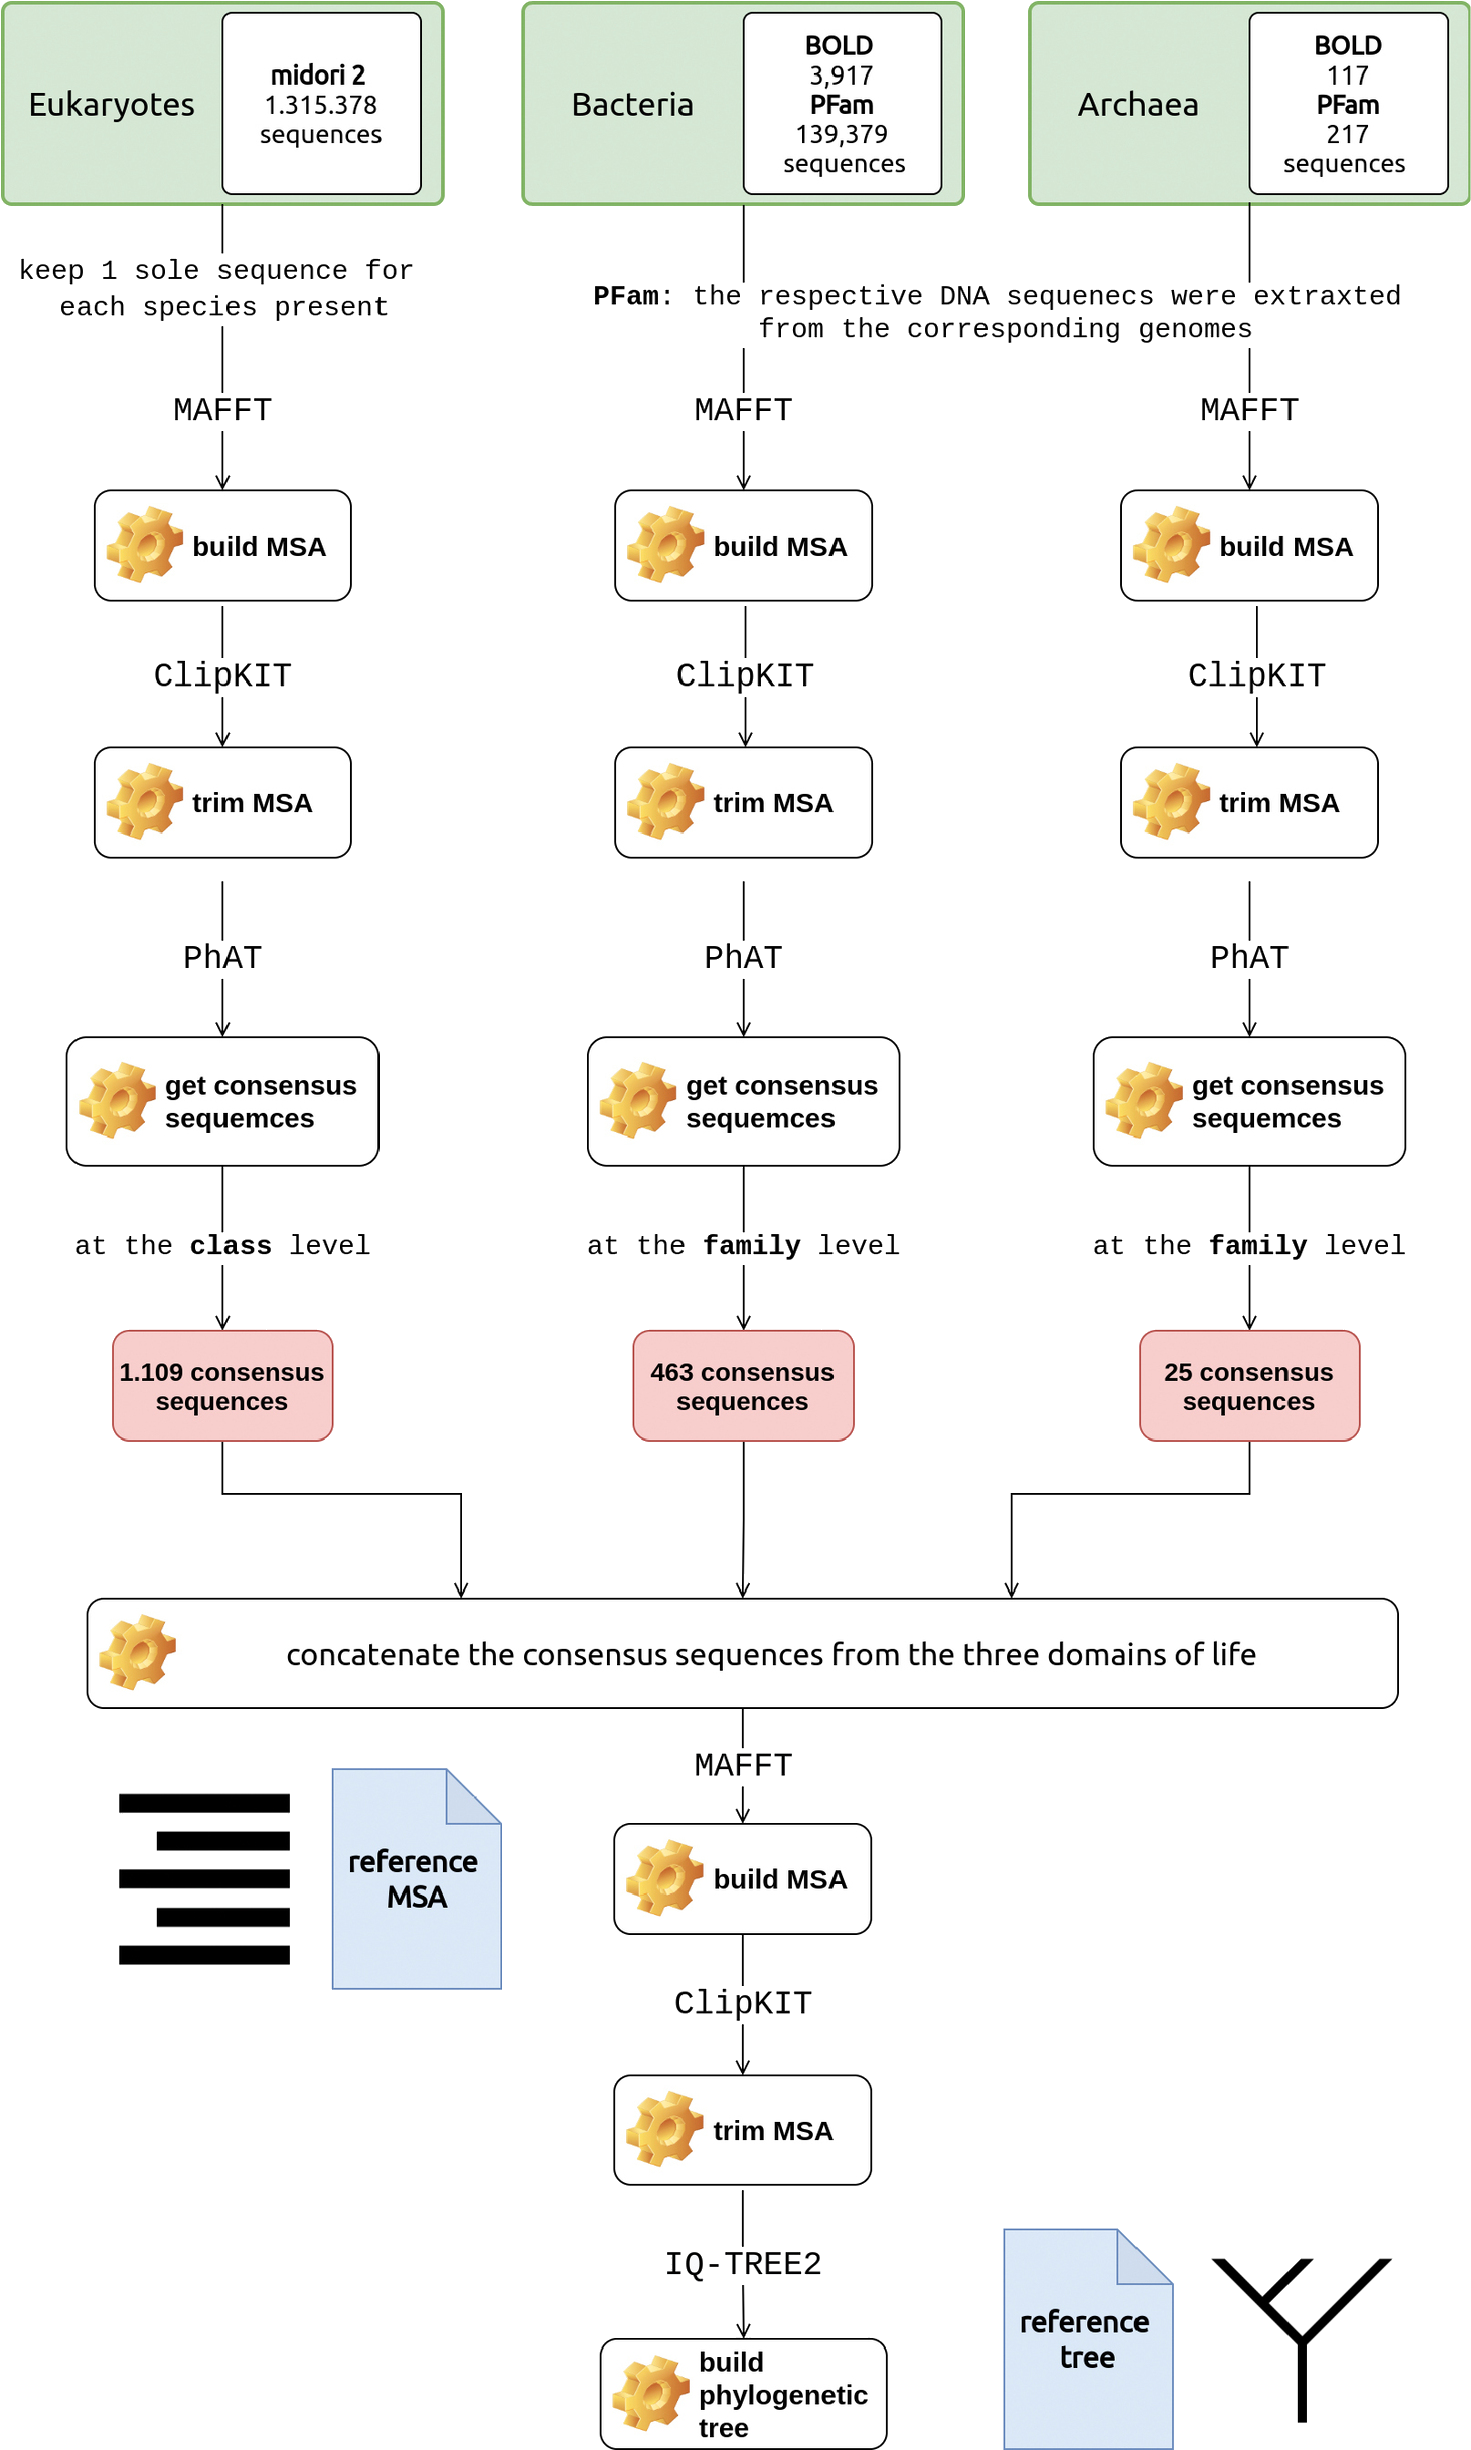
\includegraphics[width=50mm]{resources/darn_methodology_transparent.png}
   %             };
   %          \node[align = right, above, xshift=90, yshift=10] at (current page.south) {
   %             \scriptsize 
   %             Figure from: \href{https://doi.org/10.3897/mbmg.5.69657}{10.3897/mbmg.5.69657}
   %          };
   %       \end{tikzpicture}
   %    \end{singlespace}
   % \end{frame}

   % % DARN PHYLOGENY TREE
   % \begin{frame}
   %    \frametitle{Phylogeny of the COI consensus sequences retrieved}
   %    \framesubtitle{the tree that DARN makes use of}
   %    \begin{tikzpicture}[overlay, remember picture]
   %       \node[anchor=west, xshift=10pt, yshift=-15pt]
   %       at (current page.west){
   %          \includegraphics[width=60mm]{resources/placements_of_consensus_seqs_transpaernt.png}
   %       };
   %    \end{tikzpicture}

   %    \begin{textblock*}{7cm}(7.0cm, 4.5cm)
         
   %       the consensus sequences have  \\ 
   %       been placed in their corresponding \\ 
   %       taxonomic branches, proving \\
   %       the tree valid

   %    \end{textblock*}
   % \end{frame}

   % % DARN OUTPUT
   % \begin{frame}
   %    \frametitle{Bacteria are everywhere!}
   %    \framesubtitle{... Archaea too!}

   %    \begin{tikzpicture}[overlay, remember picture]
   %       \node[anchor=west, xshift=-20pt, yshift=2pt]
   %       at (current page.west){
   %          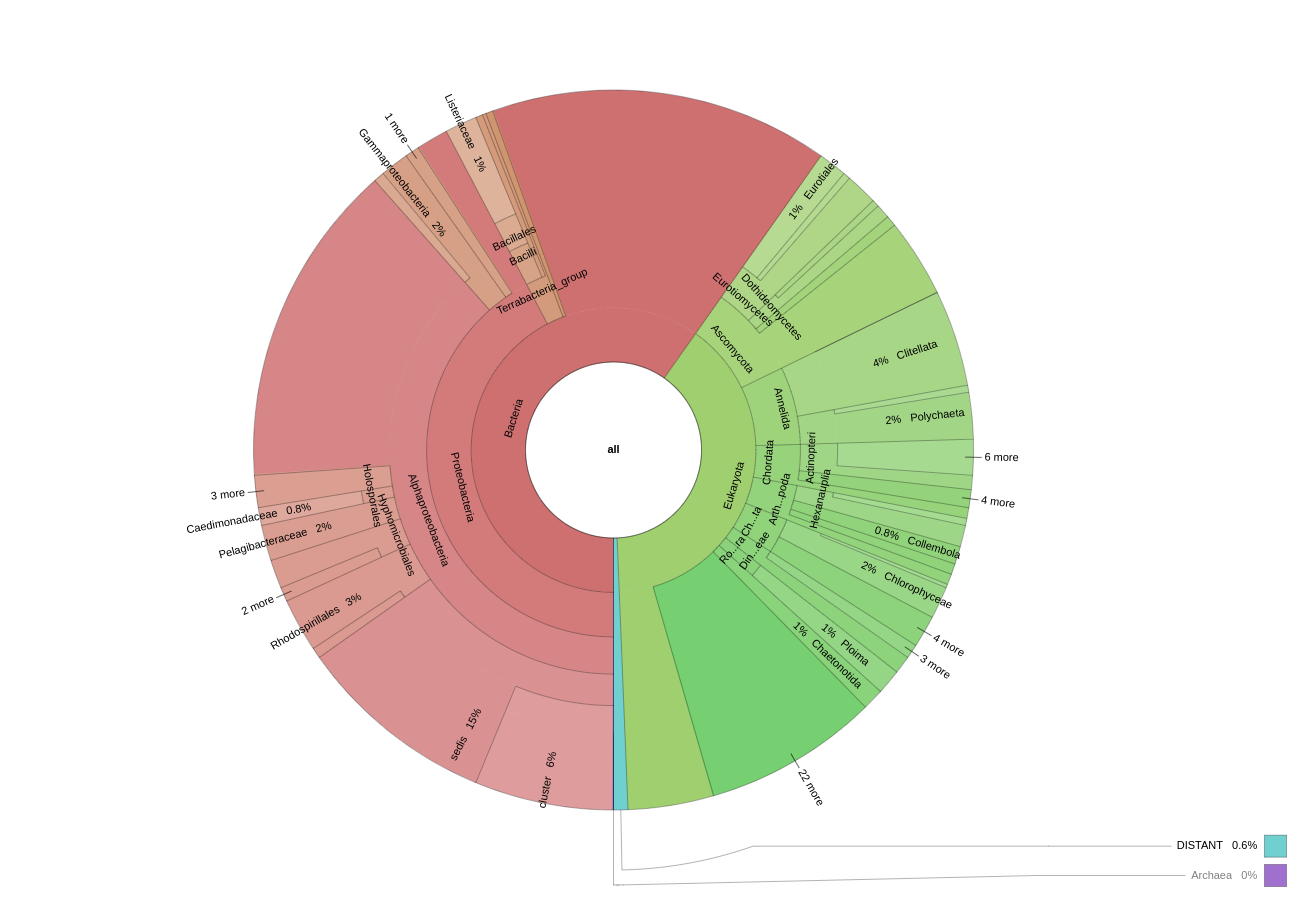
\includegraphics[width=90mm]{resources/darn_krona_output.png}
   %       };
   %    \end{tikzpicture}

   %    \begin{textblock*}{6cm}(7cm, 3.5cm)
   %       you may have a look at \\
   %       \href{https://hariszaf.github.io/darn/}{https://hariszaf.github.io/darn/} \\
   %       for more DARN output \\ 
   %       example cases
   %    \end{textblock*}

   % \end{frame}


   % -------------------------------------
   % CHANGE THE CHAPTER SLIDE: PREGO
   % -------------------------------------

   \begin{darkframes}
      \section{
         \texttt{PREGO}: a knowledge-base for organisms - environments - processes associations
      }
   \end{darkframes}

   % PREGO LOGO - SLIDE
   \begin{frame}
      
      \begin{figure}
         
\includegraphics[width=75mm]{resources/prego_logo.png}
      \end{figure}

      \begin{textblock*}{12cm}(0cm, 7cm)
         \centering
         \small related repositories under \\
         \small \href{https://github.com/orgs/lab42open-team}{https://github.com/orgs/lab42open-team} \\ 
         \small web-app under\\
         \small \href{http://prego.hcmr.gr/}{http://prego.hcmr.gr/}
      \end{textblock*}

   \end{frame}

   % PREGO VENN DIAGRAM
   \begin{frame}
      \frametitle{PREGO as \textit{processes - environments - organisms}}
      \framesubtitle{and how to link them}
      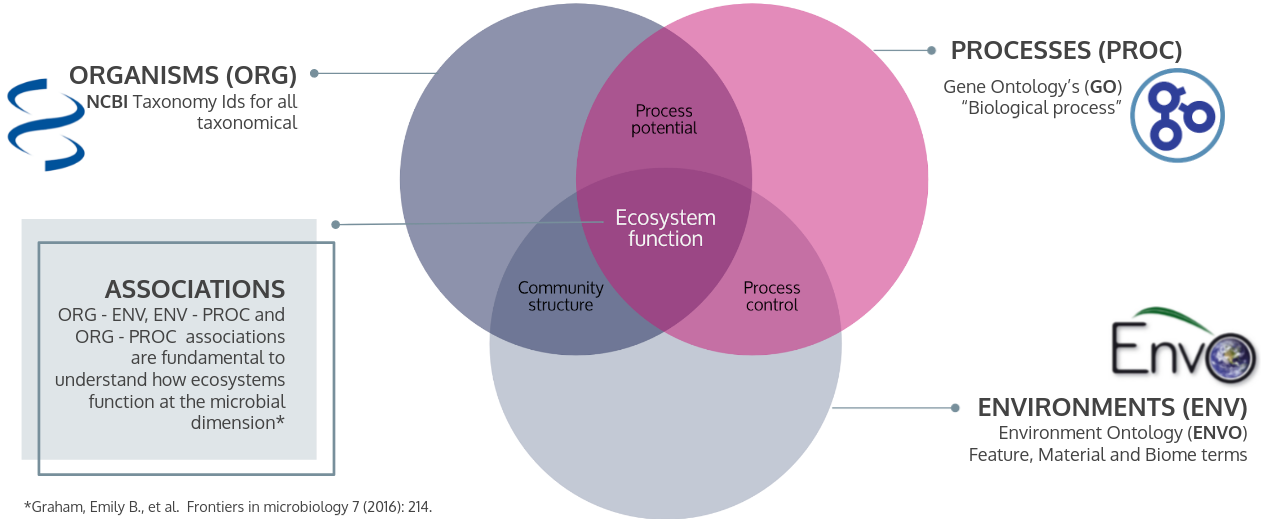
\includegraphics[width=105mm]{resources/prego_triple_associations.png}
   \end{frame}

   % METADATA
   \begin{frame}

      \frametitle{Metadata example}
      \framesubtitle{from various metagenome repositories}
      \begin{tikzpicture}[overlay,remember picture]
         \node[anchor=west, xshift=10pt, yshift=-5mm]
            at (current page.west) {
               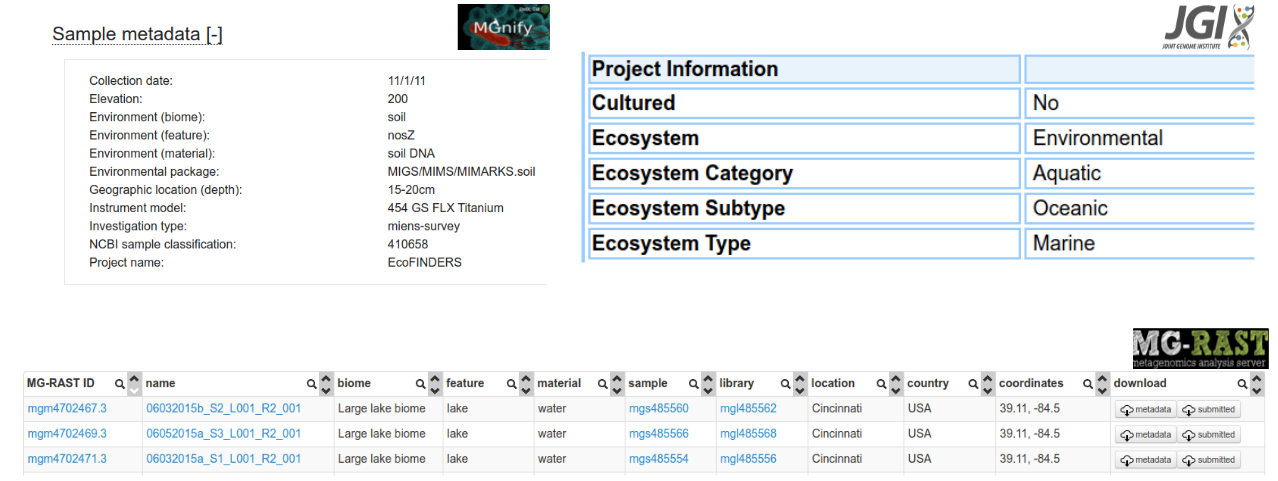
\includegraphics[width=120mm]{resources/metadata_like.png}
            };
         \end{tikzpicture} 
   \end{frame}

   % EXTRACT EXAMPLE
   \begin{frame}
      \frametitle{Named Entity Recognition}
      \framesubtitle{tagging the literature}
      \begin{figure}
         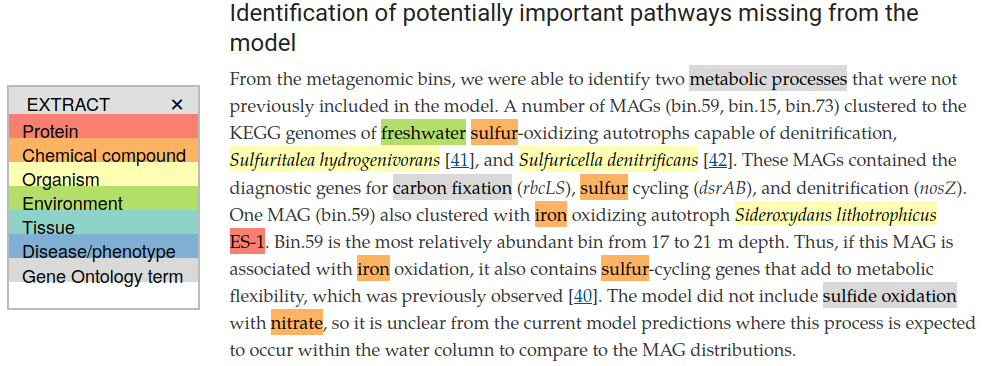
\includegraphics[width=105mm]{resources/extract_example_transp.png}
         \caption{
            \scriptsize Example text from Arora-Williams et al. Microbiome 6.1 (2018): 1-16.
         }
      \end{figure}
      
   \end{frame}

   % PREGO METHODOLOGY
   \begin{frame}

      \frametitle{PREGO methodology}
      \framesubtitle{co-occurrence again!}

      \begin{singlespace}
         \begin{tikzpicture}[overlay,remember picture]
            \node[anchor=north west, xshift=30pt,yshift=-70pt]
               at (current page.north west) {
                  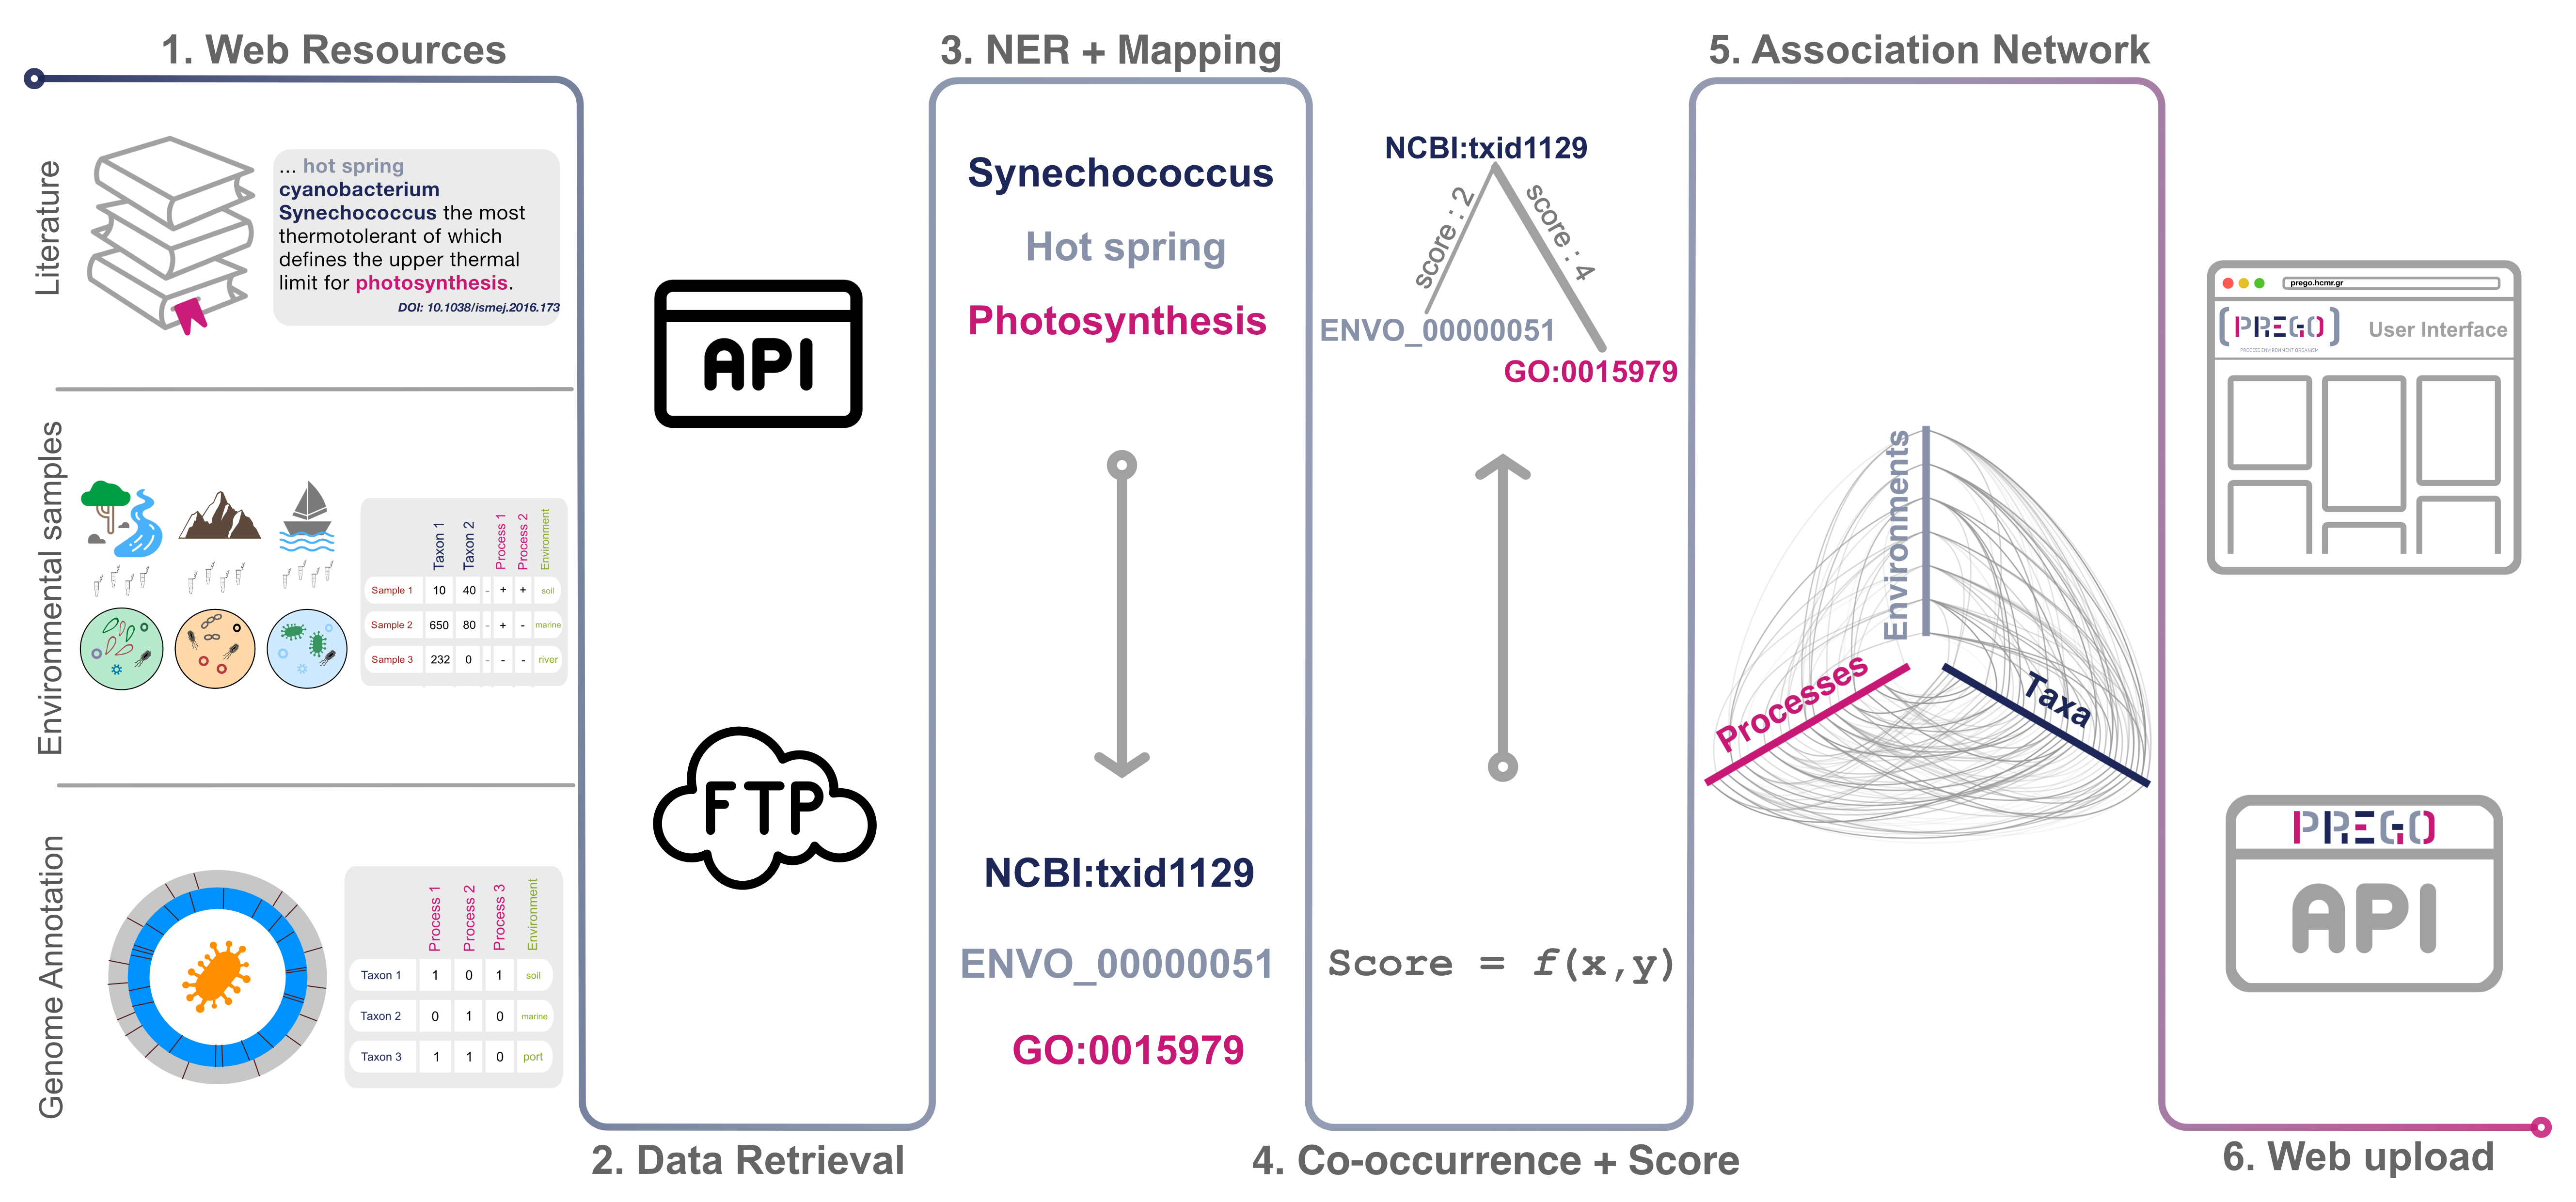
\includegraphics[width=105mm]{resources/figure_1_prego_analysis_horizontal_tr.png}
               };
            \node[align = left, above, yshift=30] at (current page.south) {
               \scriptsize 
               Figure from the PREGO publication that is now
               under review. 
               % at Special Issue  \\  
               % \scriptsize
               % "Selected Papers from the 9th Conference of the Hellenic Scientific Society MIKROBIOKOSMOS"
            };
         \end{tikzpicture}
      \end{singlespace}
   \end{frame}

   % DEVOPS
   \begin{frame}

      \frametitle{Building a knowledge-base}
      \framesubtitle{development and information technology operations}

      \begin{tikzpicture}[overlay,remember picture]
         \node[anchor=south west, xshift=10pt,yshift=30pt]
            at (current page.south west) {
               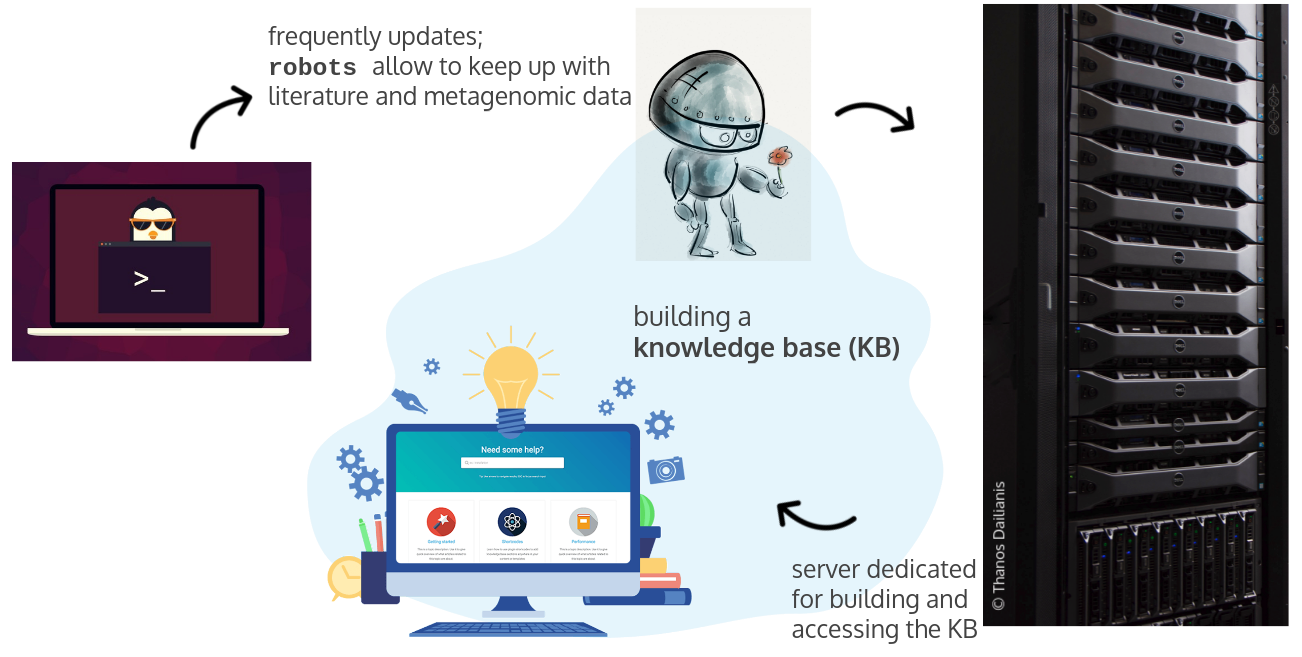
\includegraphics[width=120mm]{resources/prego_boots.png}
            };

            \node[anchor=south west, xshift=5pt,yshift=5pt]
            at (current page.south west) {
               
\includegraphics[width=35mm]{resources/devops.png}
            };
      \end{tikzpicture}
   \end{frame}

   % PREGO EXAMPLE
   \begin{frame}
      \frametitle{PREGO in action}
      \framesubtitle{looking for environments a taxon is present}

      \begin{tikzpicture}[overlay,remember picture]

         \node[anchor=west, xshift=5pt,yshift=10pt]
               at (current page.west) {
                  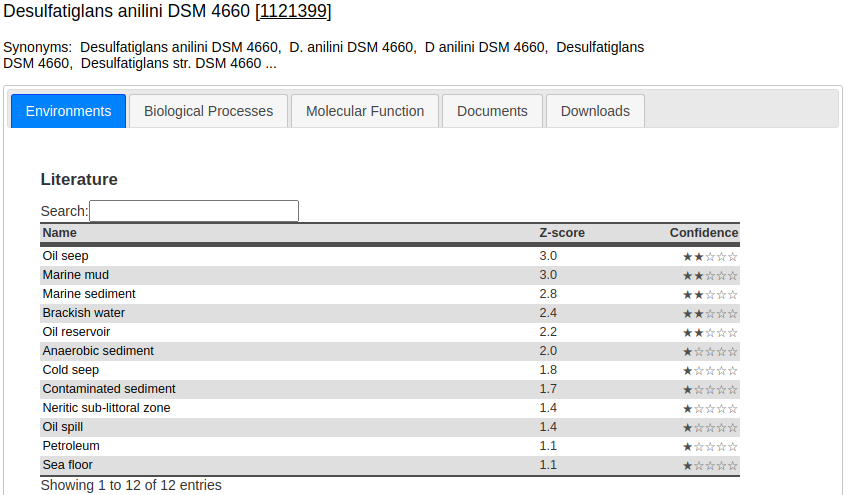
\includegraphics[width=63mm]{resources/prego_org_env_literature.png}
         };

         \node[anchor=east, xshift=-2pt,yshift=-25pt]
         at (current page.east) {
            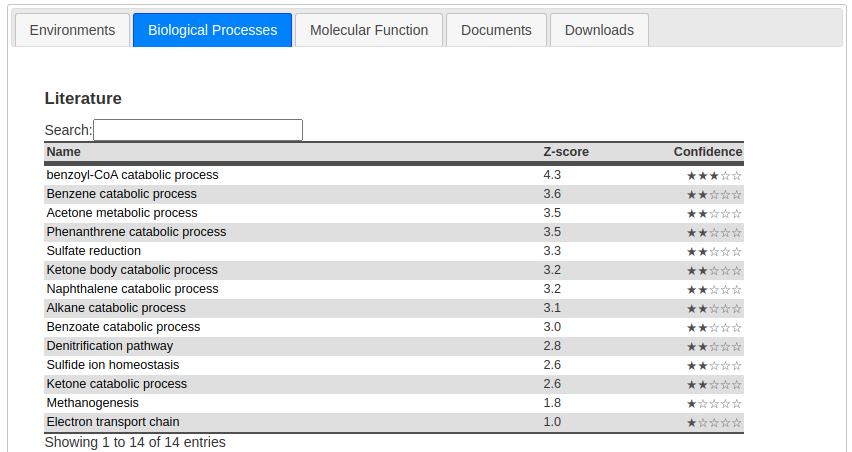
\includegraphics[width=65mm]{resources/prego_org_biol_proc_literature.png}
         };

      \end{tikzpicture}

      \begin{textblock*}{6cm}(1.0cm, 8.0cm)
         \small The PREGO knowledge-base is available at \href{http://prego.hcmr.gr/}{http://prego.hcmr.gr/}.
      \end{textblock*}

   \end{frame}


   % SLIDE FOR MARIKAT
   \begin{frame}
      \frametitle{What about taxa or functions of your interest?}
      \framesubtitle{or even environments!}

      \begin{singlespace}
         \begin{columns}[onlytextwidth]

            \column{.5\textwidth}
               \begin{tikzpicture}[overlay,remember picture]

                  \node[align = left, above, xshift=85, yshift=-40] at (current page.west) {
                     Uranium bioremedation  \\

                     by adding high \\
                     
                     concentrations of acetate \\

                     What taxa support \\
                     \textbf{\textit{"Response to acetate"}} \\
               
                     \href{https://prego.hcmr.gr/PregoAnalysis?knowledge=10&experiments=10&textmining=10&type1=-21&id1=GO:0010034}{Have a look!} \\
               
                     \textit{Geobacter} is the first hit !
               
                  };
      
               \end{tikzpicture}



            \column{.5\textwidth}
               \begin{tikzpicture}[overlay,remember picture]


                  \node[align = right, above, xshift=75, yshift=45] at (current page.south) {
                     \small
                     What about \textbf{\textit{Posidonia}} ? \\
                     \small
                     Literature suggests that Planctomycetes \\
                     \small
                     and especially \textit{Blastopirellula} \\
                     \small
                     and \textit{Rhodopirellula} are commonly \\
                     \small 
                     found in its microbiome. \\
                     Why so ? \\
                     \small
                     You may have a look \href{https://prego.hcmr.gr/PregoAnalysis?knowledge=10&experiments=10&textmining=10&type1=-2&id1=265488}{here}

                  };

               \end{tikzpicture}
         \end{columns}
      \end{singlespace}

   \end{frame}


   % -------------------------------------
   % CHANGE THE CHAPTER SLIDE: DINGO
   % -------------------------------------

   \begin{darkframes}
      \section{
         \texttt{dingo}: a Python library for metabolic flux sampling
      }   
   \end{darkframes}

   % DINGO LOGO - SLIDE
   \begin{frame}
      
      \begin{figure}
         
\includegraphics[width=55mm]{../met_nets/resources/dingo5_transparent.png}
      \end{figure}

      \begin{textblock*}{12cm}(3.5cm, 7cm)
         \href{https://github.com/GeomScale/dingo}{https://github.com/GeomScale/dingo}
      \end{textblock*}

   \end{frame}

   % A toy species model
   \begin{frame}
      \frametitle{Metabolic modelling}
      \framesubtitle{and the biomass function}
      \begin{singlespace}
         \begin{tikzpicture}[overlay,remember picture]
            \node[anchor=north west, xshift=20pt,yshift=-50pt]
               at (current page.north west) {
                  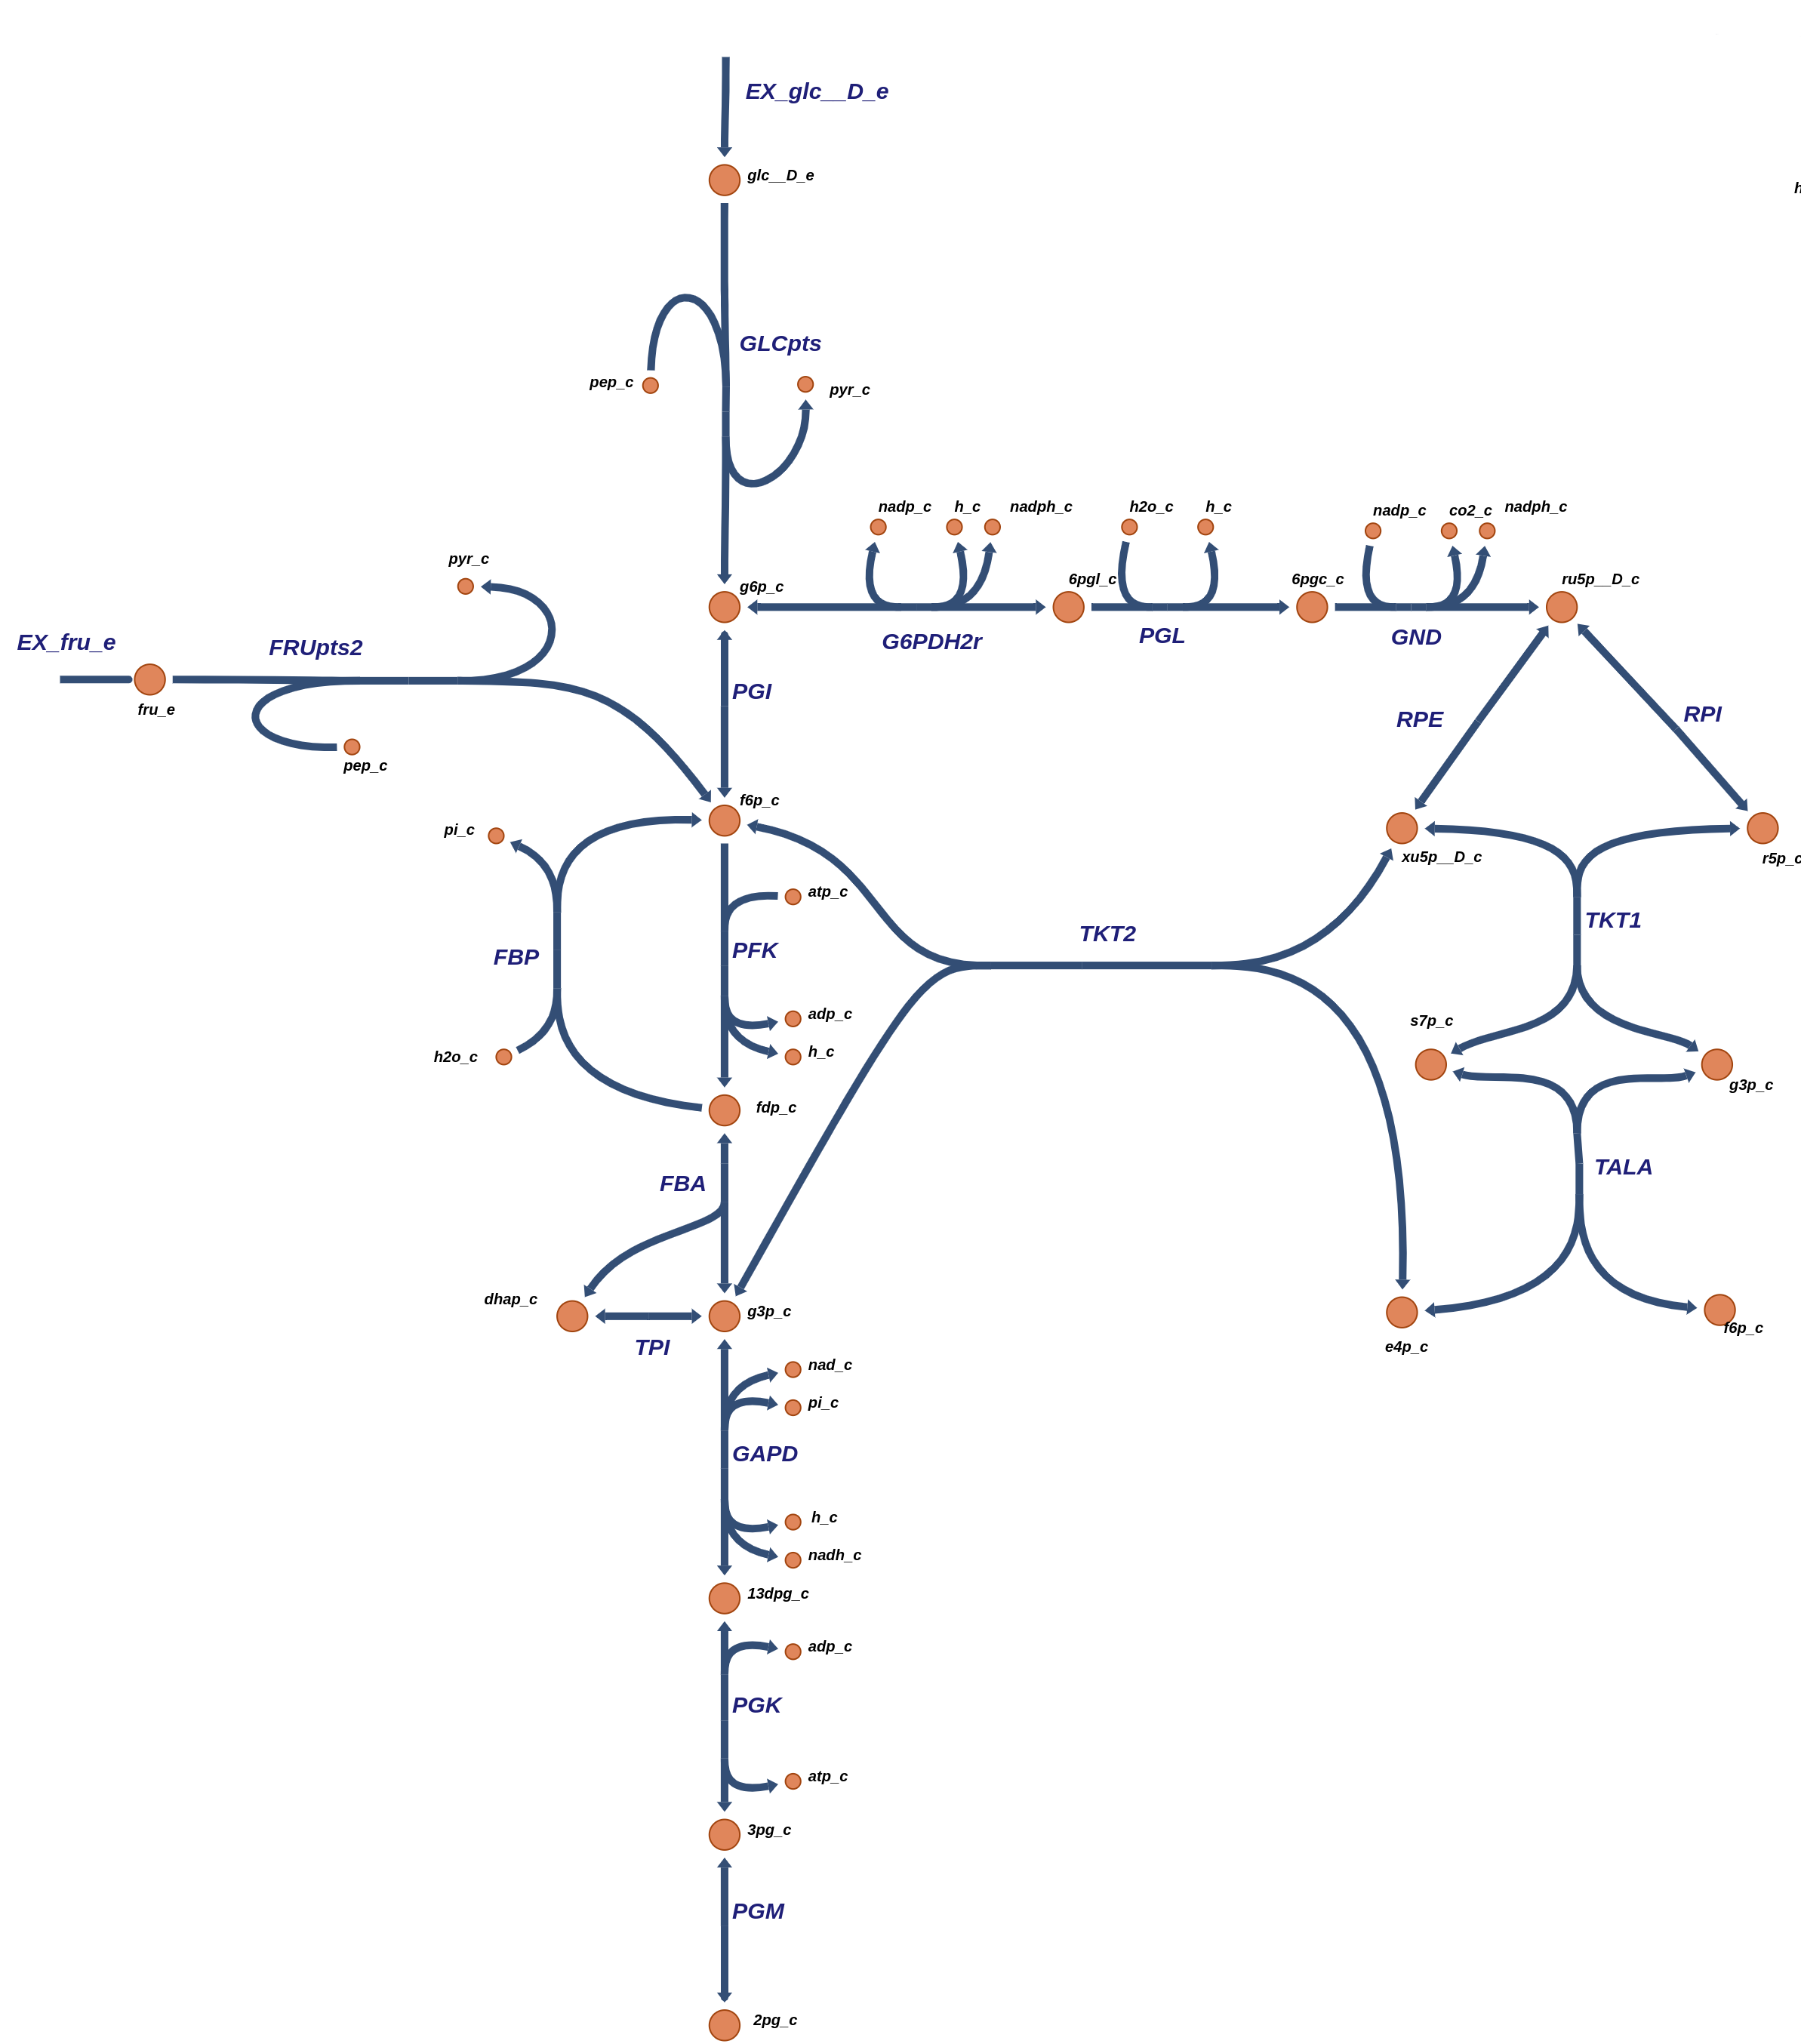
\includegraphics[width=65mm]{resources/e_coli_map_crop_Transp.png}
               };

            \node[anchor=north west, xshift=120pt,yshift=-190pt]
               at (current page.north west) {
                  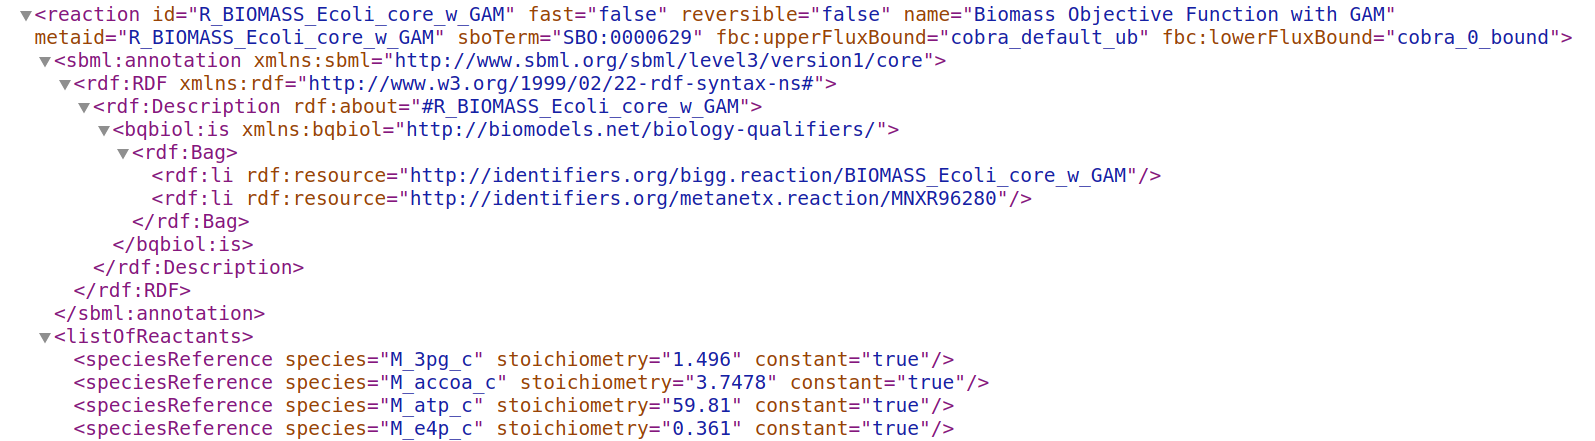
\includegraphics[width=85mm]{resources/fraction_of_Ecoli_xml_transp_crop.png}
               };
            \node[align = left, above, xshift=-80, yshift=10] at (current page.east) {
                  
                  \footnotesize Metabolic models allow us \\ 
                  \footnotesize to move from a metabolic map \\ to mathematical structures \\
                  \footnotesize the study of which may provide \\ 
                  \small fundamental biological insight
               };

         \end{tikzpicture}
      \end{singlespace}

      % SAY THAT 
      % The overall approach is to mechanistically represent the relationship between genotype and phenotype 
      % by mathematically and computationally modeling the constraints that are imposed on the
      % phenotype of a biochemical system by physicochemical laws, genetics, and the environment

   \end{frame}

   \if 0 
   % MOVING FROM ODEs TO CONSTRAINT MODELING
   \begin{frame}
      \frametitle{From concentrations to fluxes}
      \framesubtitle{to study changing environments}

      We can describe the mass balance of a chemical compound as the difference between the sum of the 
      fluxes of all the reactions that form it and the sum of all that degrade it. 

      \bigskip 

      $\frac {d\omega_i}{dt} = \sum \limits_{k} s_{ik} v_k =  \langle  s_{i} , v \rangle  $

      \bigskip

      and thus:

      \bigskip 

      $\frac {d\omega}{dt} = Sv$

   \end{frame}
   \fi

   % BUILDIING MODELS
   \begin{frame}
      \frametitle{Genome-scale metabolic reconstruction}
      \framesubtitle{approaches, pros and cons}      
      \begin{singlespace}
         \begin{tikzpicture}[overlay,remember picture]
            \node[anchor=north west, xshift=30pt,yshift=-60pt]
               at (current page.north west) {
                  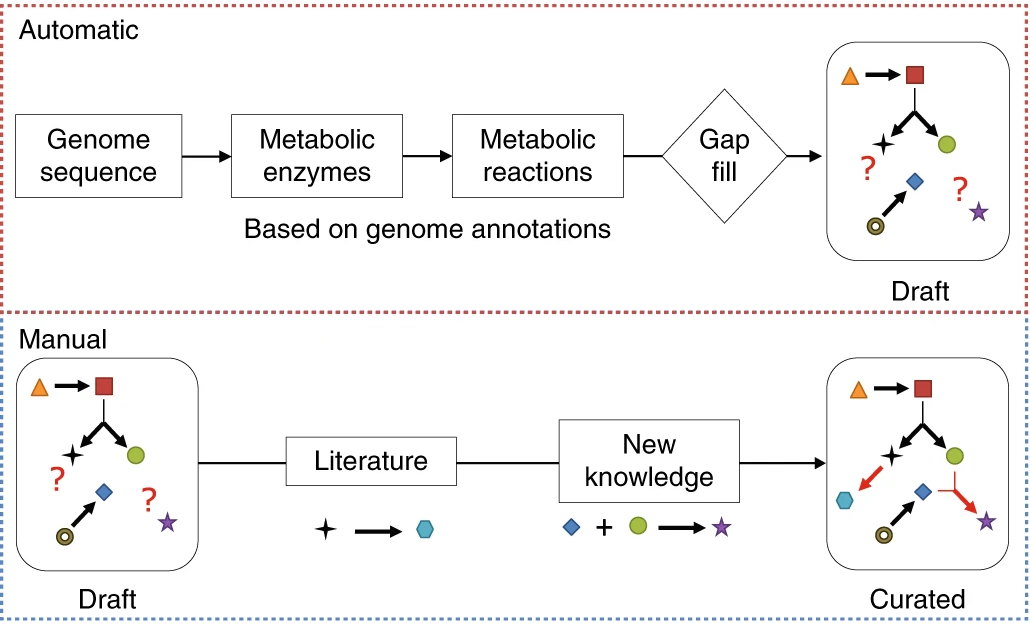
\includegraphics[width=105mm]{ ../met_nets/resources/building_gmd_transparent.png}
               };
            \node[align = left, above, yshift=10] at (current page.south) {
               \scriptsize 
               Figure from: Heirendt et al. Nature protocols 14.3 (2019): 639-702.
            };
         \end{tikzpicture}
      \end{singlespace}
   \end{frame}
   
   % STOICHIOMETRIC MATRIX & FBA
   \begin{frame}{From a stoichiometric matrix}
      \framesubtitle{to a constraint-based model}
      
      \begin{singlespace}
         \begin{tikzpicture}[overlay,remember picture]

            \node[anchor=north west, xshift=20pt,yshift=-65pt]
               at (current page.north west) {
                  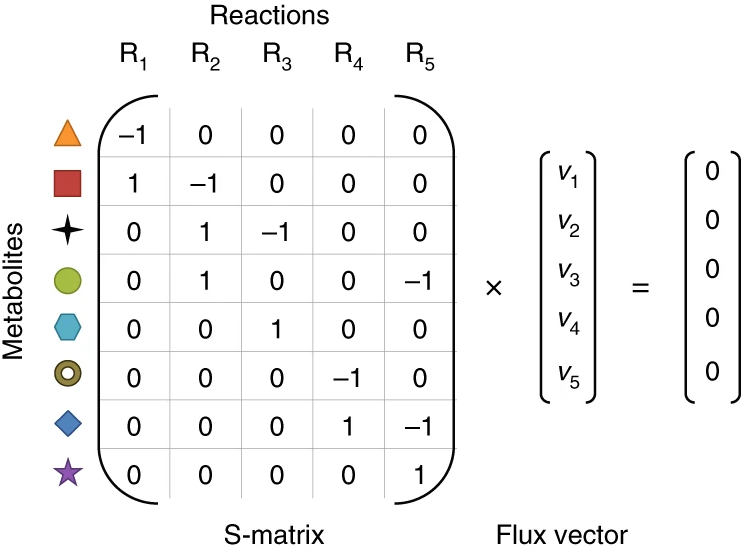
\includegraphics[width=70mm]{ ../met_nets/resources//stoichiometric_matrix_transparent.png}
               };

               \node[align = left, above, yshift=10] at (current page.south) {
                  \scriptsize 
                  Figure from: Heirendt et al. Nature protocols 14.3 (2019): 639-702.
               };
   
            \node[align = center, left, xshift=-10pt] at (current page.east) {
               \footnotesize In a \textbf{steady state} \\
               \footnotesize the production rate \\
               \footnotesize of each metabolite \\ \bigskip
               \footnotesize equals its consumption rate \\  

               \footnotesize The \textbf{flux vector}
               \footnotesize is a vector with \\
               \footnotesize the value of \\
               \footnotesize each reaction flux \\
               \footnotesize in a certain steady \\ \bigskip
               \footnotesize state. \\  

               \footnotesize The steady state assumption \\
               \footnotesize is ensured by \\
               \footnotesize the \textbf{zero-vector}. 

               % \textbf{Flux Balance Analysis}
               % \\ 
               % \small
               % Maximize \/ minimize an \\
               % \small
               % objective function:  \\
               % \small
               % $\psi = c_1 v_1 + c_2 v_2 + .. + c_5 v_5$ \\
               % \small
               % such that: \\
               % \small
               % $S  v = O$ \\ 
               % \small
               % and for each reaction $i$: \\
               % \small
               % $lb_i \leq v_i \leq ub_i$ \\ 
               
               % \\

               % \small
               % where $lb$: lower bound, \\
               % \small
               % $ub$: upper bound and \\
               % \small
               % $S$: the stoichiometric matrix
            };

         \end{tikzpicture}
      \end{singlespace}      
   \end{frame}

   % GET FULL DIM POLYTOPE
   \begin{frame}
      \frametitle{The region of steady states}
      \framesubtitle{moving to full dimensional polytope}

      \begin{columns}[onlytextwidth]

         \column{.4\textwidth}
         \centering

            \small
            The \textit{constraints} on the reactions fluxes.
             \begin{equation}
               \begin{split}
                Sv=0, \\ 
                v_{lb} \leq v \leq v_{ub}
               \end{split}
            \label{eq:fba}
            \end{equation}
 

            \bigskip
            $S \in \mathbb{R}^{m \times n}, v \in \mathbb{R}^{n}$


         \column{0.2\textwidth}
         \centering
            $\underleftrightarrow{v = Nx}$

         \column{.4\textwidth}
         \centering

            As a \textit{full dimensional} polytope

            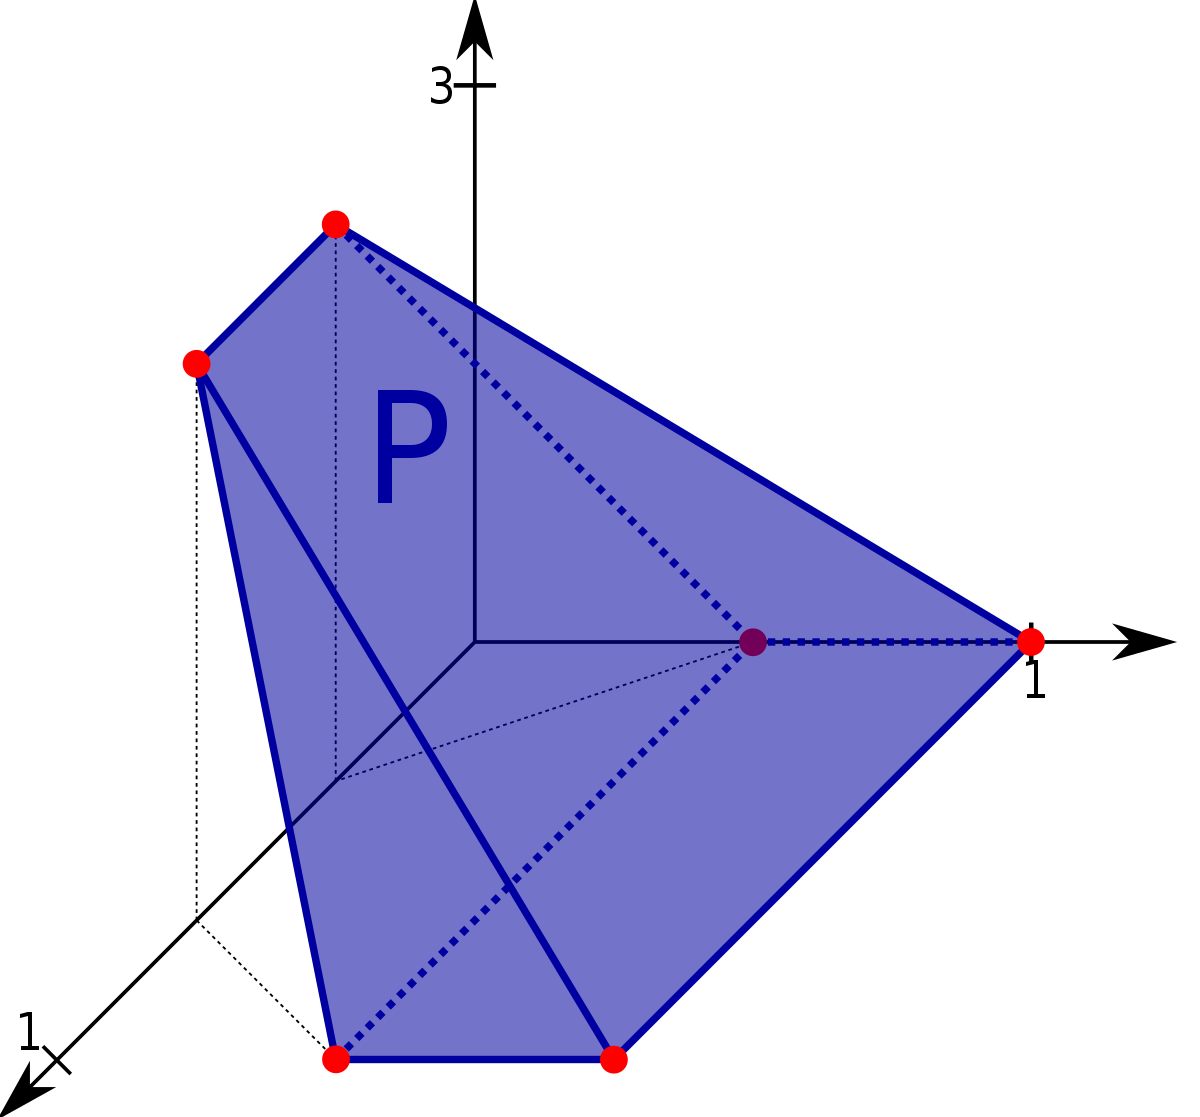
\includegraphics[width=30mm]{../met_nets/resources/3dpoly.svg.png}

            $P := \{x \in \mathbb{R}^d | Ax \leq b\}$

      \end{columns}

      \bigskip

      \footnotesize
      $N\in\mathbb{R}^{n\times d}$ denotes the matrix of the null space of $S$,
      i.e. $S N = 0_{m \times d}$. \bigskip

      \footnotesize
      By replacing $v$ with $Nx$ in Equation~\ref{eq:fba}, we get the full dimensional polytope $P$,  
      where 
      $A = \begin{pmatrix} I_n N \\ -I_n N\end{pmatrix}$
      and 
      $b = \begin{pmatrix} v_{ub} \\ v_{lb} \end{pmatrix}  N$, (in $\mathbb{R}^d$).

   \end{frame}


   % FLUX SAMPLING
   \begin{frame}[label=simmonshall]{Flux sampling} 

      \framesubtitle{an alternative approach}
      \begin{singlespace}
         \begin{tikzpicture}[overlay,remember picture]

            \node[anchor=north west, xshift=30pt,yshift=-60pt]
               at (current page.north west) {
                  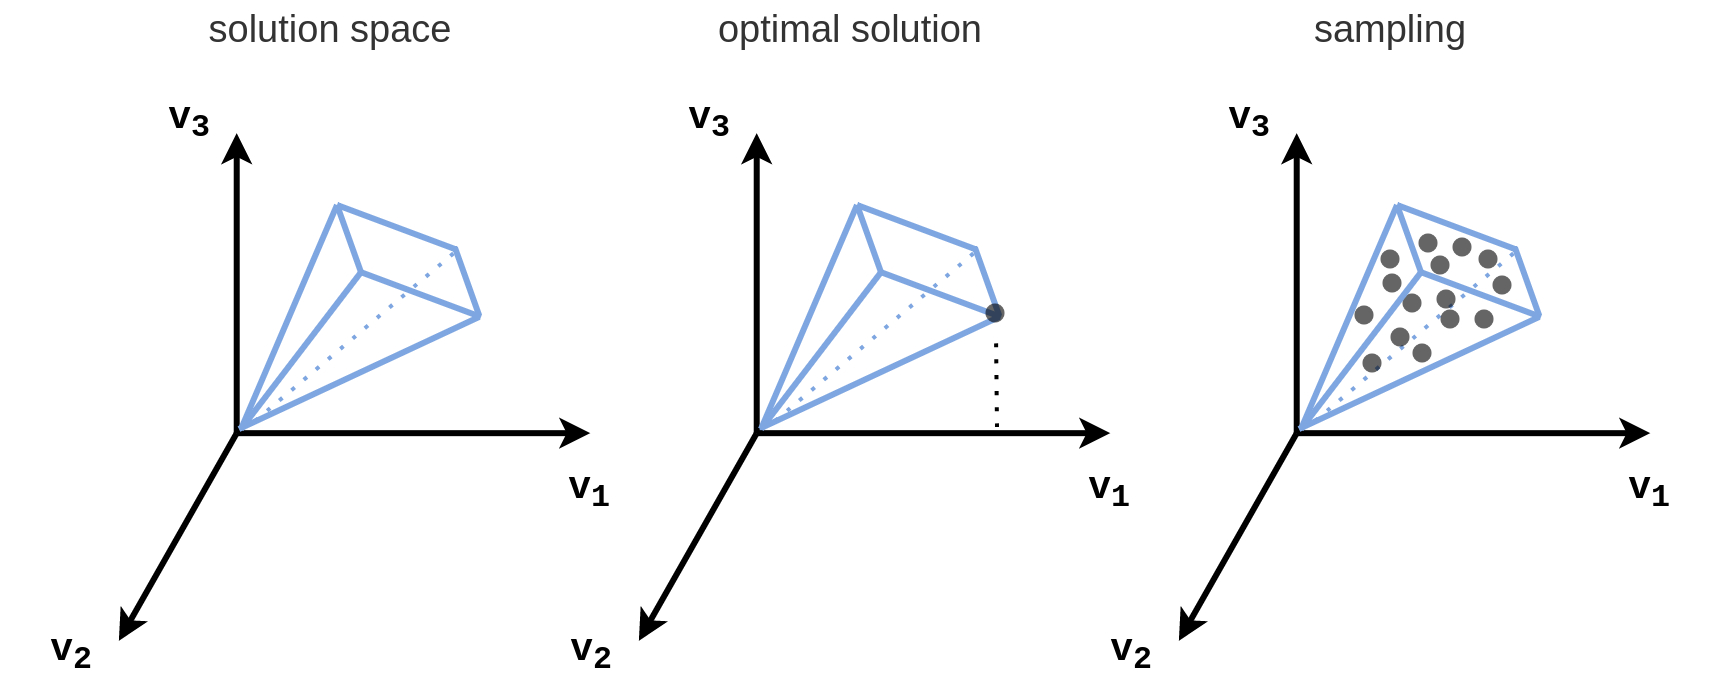
\includegraphics[width=100mm]{ ../met_nets/resources/space_fba_sampling.png}
               };

               % \node[align = left, above, yshift=10] at (current page.south) {
               %    \scriptsize 
               %    Figure from: Heirendt et al. Nature protocols 14.3 (2019): 639-702.
               % };

            \end{tikzpicture}

         \bigskip  \justifying  \bigskip
         \bigskip  \justifying  \bigskip
         \bigskip  \justifying  \bigskip

            \begin{itemize}
               \item \small 
               enables the analysis of GEMs without the need of an objective function
               \item \small
               determines the feasible solution spaces for fluxes in a network based on a set of conditions as well as the probability of obtaining a solution               
            \end{itemize}

      \end{singlespace}
   \end{frame}

   % make a slide for the sampling performance metrics
   % these are: 
   %  - cost per iteration: the number of operations the algorithm needs to sample a single point
   %  - mixing time: the number of samples the algorithm needs to burn in order to lose dependency from previous iterations (i.i.d)
   %  - cost per sample: the total number of operations the algorithm needs to sample an i.i.d point


   % BILLIARD WALK
   \begin{frame}
      \frametitle{Billiard walk}
      \framesubtitle{for random sampling}

      \begin{columns}[t, totalwidth=7cm]

         \column{.3\textwidth}
            
\includegraphics[width=27mm]{../met_nets/resources/bill1.png}

         \column{.3\textwidth}
            \includegraphics[width=27mm]{../met_nets/resources/bill2.png}

      \end{columns}

      \bigbreak


      \begin{columns}[t, totalwidth=7cm]

         \column{.3\textwidth}
            \includegraphics[width=27mm]{../met_nets/resources/bill3.png}

         \column{.3\textwidth}
            \includegraphics[width=27mm]{../met_nets/resources/bill4.png}

      \end{columns}

      \bigbreak

      \begin{columns}[t, totalwidth=7cm]

         \column{.3\textwidth}
            \includegraphics[width=27mm]{../met_nets/resources/bill5.png}

         \column{.3\textwidth}
            \includegraphics[width=27mm]{../met_nets/resources/bill6.png}

      \end{columns}

      \begin{textblock*}{8.0cm}(8.5cm, 3.0cm)
         \footnotesize Generate the length of the \\ trajectory $L \sim D$. \\
         \bigbreak
         \footnotesize Pick a uniform direction $v$ \\ to define the trajectory. \\
         \bigbreak
         \footnotesize The trajectory reflects on \\ the boundary if necessary. \\
         \bigbreak
         \footnotesize Return the end of the \\ trajectory as $p_i+1$.
      \end{textblock*}

   
   \end{frame}

   % When the polytope is skinny:
% The average number of reflections increases.
% The mixing rate decreases.


   % MCMC ALGORITHM
   \begin{frame}{Our Markov Chain Monte Carlo (MCMC) algorithm}
      \framesubtitle{for flux sampling}

      \includegraphics[scale=0.11]{ ../met_nets/resources//sampling_extra_phase_croped_transparent.png}
      
      \scriptsize
      \begin{block}{Steps of an MMCS phase}
         \begin{itemize}
            \item \textbf{sampling step:} using a variant of the \textbf{Billiard walk}  
            \item \textbf{rounding step:} calculate a linear transformation $T_i$ that puts the sample into isotropic position and then apply it on $P_i$ to obtain the polytope of the next phase
            \item check several statistic tests
         \end{itemize}      

      \end{block}

      % \begin{singlespace}
      %    \scriptsize
      %    Chalkis, Fisikopoulos, Tsigaridas and Zafeiropoulos 
      %    "Geometric Algorithms for Sampling \\ the Flux Space
      %    of Metabolic Networks", SoCG 2021,  
      %    DOI: 10.4230/LIPIcs.SoCG.2021.21
   
      % \end{singlespace}

   \end{frame}

   % RENZ ET AL. PAPER
   % \begin{frame}{Find possible targets against SARS-CoV-2}
   %    \framesubtitle{a flux sampling application}
   %    \bigskip
   %    \includegraphics[scale=0.27]{ ../met_nets/resources//covid_paper.png}
      
   %    \begin{singlespace}
   %       \begin{itemize}
   %          \item \small Renz et al. '20 built the biomass function of Sars-Cov-2 to build a host - virus network
   %          \item \small Using FBA they computed an optimal steady state using \\ \small \quad (i) human biomass maintenance,\\ \small \quad (ii) virus growth rate
   %          \item \small They found reaction GK1 as a possible anti-viral target.
   %       \end{itemize}            
   %    \end{singlespace}

   % \end{frame}


   % SAMPLING ON THE RENZ ET AL. MODEL 
   \begin{frame}{Find possible targets against SARS-CoV-2}
      \framesubtitle{a flux sampling application}      

      \begin{tikzpicture}[overlay,remember picture]

         \node[anchor=north east, xshift=-10pt,yshift=-30pt]
            at (current page.north east) {
               \includegraphics[width=20mm]{ ../met_nets/resources//dingo5_transparent.png}
            };
      \end{tikzpicture}


      \centerline{
      \includegraphics[scale=0.21]{
          ../met_nets/resources//density_flux_TYMSULT_fba_2_transparent
         } 
      \includegraphics[scale=0.21]{
          ../met_nets/resources//density_flux_gk1_fba_2_transparent
         }
      }

      \begin{itemize}
         \item Check if the flux distribution of a reaction changes.
         \item Find possible anti-viral targets and study further.
      \end{itemize}
      \vspace*{0.2cm}

   \end{frame}

   % COPULA
   \begin{frame}
      \frametitle{What is the probability of a flux value of a reaction}
      \framesubtitle{with respect to the flux value of another reaction}
      \centering
      \includegraphics[width=95mm]{resources/hex_-_g6pper_transp.png}
   \end{frame}

   % FLUX SAMPLING APPLICATIONS
   \begin{frame}{Further applications}
      \framesubtitle{of metabolic flux sampling}

      \begin{singlespace}

         \begin{columns}[onlytextwidth]

            \column{.5\textwidth}
               \begin{tikzpicture}[overlay,remember picture]
                  
                  \node[anchor=north west, xshift=15, yshift=-100pt]
                  at (current page.north west) {
                     \includegraphics[width=55mm]{ ../met_nets/resources//cartoon_wine.jpg}

                  };

                  \node[align = left, above, xshift=-80, yshift=35] at (current page.south) {
                     \scriptsize Scott, William T., et al. "Metabolic flux sampling \\ 
                     \scriptsize predicts strain-dependent differences related to \\ 
                     \scriptsize 
                     aroma production among commercial wine yeasts." \\
                     \scriptsize
                      Microbial cell factories 20.1 (2021): 1-15.   
                  };
      
               \end{tikzpicture}



            \column{.5\textwidth}
               \begin{tikzpicture}[overlay,remember picture]

                  \node[anchor=north east, xshift=-45, yshift=-100pt]
                     at (current page.north east) {
                        \includegraphics[width=30mm]{ ../met_nets/resources//interactions_transparent.png}
                     };

                  \node[align = right, above, xshift=95, yshift=65] at (current page.south) {
                     \small
                     What about microbial interactions ? 
                  };
                  % \node[align = right, above, xshift=-20, yshift=35] at (current page.south) {

                  %    fsfasfhasdf

                  % }

               \end{tikzpicture}
         \end{columns}
      \end{singlespace}
   \end{frame}

   % % dingo Python library
   % \begin{frame}{\texttt{dingo}: a Python library }
   %    \framesubtitle{for flux sampling}

   %    \begin{columns}[onlytextwidth]

   %       \column{.48\textwidth}
   %          \includegraphics[scale=0.1]{ ../met_nets/resources//dingo5_transparent.png}
         
   %          \href{https://github.com/GeomScale/dingo}{https://github.com/GeomScale/dingo}

   %       \column{.41\textwidth}

   %          \begin{center}
   %             \texttt{how to} GCollab notebook
   %             \includegraphics[scale=0.3]{ ../met_nets/resources//dingo_collab_transparent.png}               
   %          \end{center}
 
   %    \end{columns}

   % \end{frame}


   % -------------------------
   % CHANGE THE CHAPTER SLIDE: TRISTOMO SWAMP 
   % -------------------------
   % \begin{darkframes}
   %    \section{
   %       Tristomo swamp: a hybrid amplicon \& shotgun metagenomics analysis 
   %    }
   % \end{darkframes}


   % \begin{frame}
   %    \frametitle{A swamp in Karpathos}
   %    \framesubtitle{an Aegean island}
   %    \includegraphics[width=85mm]{resources/tristomo_swamp.png}
   % \end{frame}


   % -------------------------------------
   % CHANGE THE CHAPTER SLIDE: HPC
   % -------------------------------------

   \if 0 

   \begin{darkframes}
      \section{0s \& 1s in molecular biology}
   \end{darkframes}

   % ZORBAS PROJECT RESOURCES
   \begin{frame}

      \frametitle{Computational requirements}
      \framesubtitle{for \textit{trivial} bioinformatic tasks}

      \begin{tikzpicture}[overlay, remember picture]
         \node[anchor=north, yshift=-30mm]
            at (current page.north){
               \includegraphics[width=105mm]{resources/imbbc_needs.jpeg}
            };
      \end{tikzpicture}

      \begin{textblock*}{10cm}(2cm, 7.5cm)
            \scriptsize Red bars denote published research with high resource requirements \\
            \scriptsize of the various computational methods employed at the IMBBC HPC facility
      \end{textblock*}


   \end{frame}

   % ZORBAS SCHEME
   \begin{frame}
   
      \frametitle{Zorbas: the HPC facility of IMBBC}
      \framesubtitle{a Tier 2 (regional) HPC facility}
      
      \begin{tikzpicture}[overlay, remember picture]
         \node[anchor=west, xshift=25pt, yshift=-20pt]
            at (current page.west){
               \includegraphics[width=60mm]{resources/zorbas_transp.png}
            };
         
      \end{tikzpicture}

      \begin{textblock*}{3.5cm}(8.5cm,5cm)
         Block diagram of the Zorba architecture
      \end{textblock*}
   
   \end{frame}

   % INFRASTUCTURES
   \begin{frame}
      \frametitle{Computing infrastructures}
      \framesubtitle{an alternative for the most!}
   
      \begin{tikzpicture}[overlay,remember picture]

         \node[anchor= west, xshift=10pt]
            at (current page.west){
               \includegraphics[width=60mm]{resources/marine-genomic-observatories.png}
            }; 

            \node[anchor= west, xshift=10pt, yshift=-90pt]
            at (current page.west){
               \includegraphics[width=35mm]{resources/Elixir-Europe-logo-1.png}
            };

            \node[anchor= west, xshift=160pt, yshift=-90pt]
            at (current page.west){
               \includegraphics[width=50mm]{resources/lw_logo.png}
            };

      \end{tikzpicture}


      \begin{textblock*}{5cm}(7.4cm, 3.0cm)

         \small We will develop a workflow  \\
         \small for the analysis of Genomic \\ 
         \small Observatories (GOs) data \\
         \small that will allow researchers \\ 
         \small to deal better with the  \\
         \small increasing amount of data

      \end{textblock*}
   
   \end{frame}

   \fi

   \if 0
   % -------------------------------------
   % CHANGE THE CHAPTER SLIDE: MICROBETAG 
   % -------------------------------------
   \begin{darkframes}
      \section{
         \texttt{microbetag}: enhancing microbial interactions inference from co-occurrence networks
      }
   \end{darkframes}

   % MICROBETAG MODULES 
   \begin{frame}

      \frametitle{
         \texttt{microbetag}: annotating co-occurrence networks
      }
      \framesubtitle{and a trip to KU Leuven}

      \begin{textblock*}{5cm}(1.0cm, 3.5cm)
         We will try building 3 modules: 
         
         \begin{itemize}
            \small \item pathway complementarity
            \small \item environmental conditions and phenotypic data integration
            \small \item flux sampling on pairs of metabolic models (if possible)
         \end{itemize}

      \end{textblock*}

      \begin{tikzpicture}[overlay,remember picture]
         \node[anchor=north east, xshift=-5pt,yshift=-55pt]
            at (current page.north east) {
               \includegraphics[width=62mm]{resources/Sources-of-co-occurrence-in-microbial-interaction-networks-A-Cooccurrence_W640_trans.png}
            };
         
      \end{tikzpicture}

      \begin{textblock*}{7cm}(6.0cm, 7.5cm)
         \scriptsize Figure from R{\"o}ttjers \& Faust (2018). 
                     FEMS microbiology reviews. 42. 10.1093/femsre/fuy030.
      \end{textblock*}


      \begin{tikzpicture}[overlay,remember picture]
         \node[anchor=south west,
               xshift=15pt,
               yshift=22pt]
               at (current page.south west) {
                  \includegraphics[width=25mm]{
                      resources/embo_logo.png
                  }
               };

      \end{tikzpicture}



   \end{frame}

   % FIRST STEPS 1/3
   \begin{frame}
      \frametitle{First steps (1/3)}
      \framesubtitle{pathway complementarity module}

      \begin{singlespace}
         
         \begin{textblock*}{10cm}(1.0cm, 2.7cm)
            
            \begin{enumerate}
               \small \item use abundance \& metadata table to run FlashWeave
               \small \item get the NCBI Taxon id of each taxon present in the edge file
               \small \item search for available reference genomes for these ids 
               \small \item use KEGG modules to get major metabolic pathways of interest
               \small \item search for pathway complementarity in each module of interest
            \end{enumerate}

         \end{textblock*}

         \begin{textblock*}{10cm}(1.2cm, 6.0cm)

            \scriptsize Relative work \\ 
            \begin{itemize}
               \scriptsize \item \href{https://www.pnas.org/content/110/31/12804}{Levy \& Borenstein}. Proceedings of the National Academy of Sciences 110.31 (2013): 12804-12809. \\
               \scriptsize \item \href{https://www.pnas.org/content/112/20/6449.long}{Zelezniak et al.} Proceedings of the National Academy of Sciences 112.20 (2015): 6449-6454. 
            \end{itemize}

         \end{textblock*}

      \end{singlespace}

   \end{frame}

   % FIRST STEPS 2/3
   \begin{frame}
      \frametitle{First steps (2/3)}
      \framesubtitle{phenotypical annotation module}

      \begin{singlespace}
         
         \begin{textblock*}{10cm}(1.0cm, 2.7cm)
            

            \begin{enumerate}

               \setlength\itemsep{2em}


               \small \item \textbf{BugBase} to get: 
                  \begin{itemize}
                     \scriptsize \item Gram Positive \& Negative
                     \scriptsize \item Biofilm Forming
                     \scriptsize \item Pathogenic Potential
                     \scriptsize \item Mobile Element Containing
                     \scriptsize \item Oxygen Utilizing
                     \scriptsize \item Oxidative Stress Tolerant
                  \end{itemize}

               
               \small \item \textbf{FAPROTAX} database: \\
                     \scriptsize to map taxa to established metabolic or other ecologically relevant functions, using the current literature on cultured strains
                     % FAPROTAX includes software for converting taxonomic microbial community profiles (e.g. in the form of an OTU table) into putative functional profiles, based on taxa identified in a sample.
            \end{enumerate}

         \end{textblock*}


         \begin{textblock*}{5cm}(7.2cm, 3.5cm)
            \small Further annotation sources to be considered: 
            \begin{itemize}
               \small \item \href{https://bioinfo.imtech.res.in/manojk/sigmol/}{SigMol}
               \small \item \href{https://api.bacdive.dsmz.de/}{BacDive}
            \end{itemize}
      
         \end{textblock*}

      \end{singlespace}

   \end{frame}

   % FIRST STEPS 3/3
   \begin{frame}
      \frametitle{First steps (3/3)}
      \framesubtitle{ecoEFMs}

      \begin{singlespace}
         
         \begin{textblock*}{10cm}(1.0cm, 2.7cm)
            

            \centering
            \includegraphics[width=105mm]{resources/nature_nutrition.png}
            % \begin{enumerate}
            %    \small \item Reconstruct all the models (that is possible to) for the taxa present in the co-occurence network

            %    \small \item Build the medium they live in; could be a gut-like environment (Thiele et al.). or a random media (dirichlet distribution) even better (Daniel's paper - have to find it)
               
            %    \small \item Build merged paired models for each association; to do this, we will keep the model of species A and we will add all the reactions of species B that are not present in species A. As the initial model of species B has no transporters for species A by-products that does not need, then it will not affect it

            %    \small \item Get the EFMs of the merged model; to this end, source code of Daniel's will be exploited; specifically:
               
            %       \begin{itemize}
            %          \item the \texttt{create_panReactome_model.py} will be edited for the case of eco models likewise, the get_PanEFMs.py will be modified accordingly
            %          \item the ecoEFMs will be extracted and various scores will be computed; e.g., tha ration between the ecoEFMs of species A / total EFMs.
            %       \end{itemize}
               
            %    \small \item The ecoEFMs that icnlude a seed node will be annotated as super valid association

            % \end{enumerate}

         \end{textblock*}

      %    \begin{textblock*}{10cm}(1.2cm, 6.0cm)

      %       \scriptsize Bibliography \\ 
      %       \begin{itemize}
      %          \scriptsize  lslkdjf
      %       \end{itemize}

      %    \end{textblock*}

      \end{singlespace}

   \end{frame}

   % TOOLS AND DBs TO EXPLOIT
   \begin{frame}
      \frametitle{Databases to exploit}
      \framesubtitle{and how to}

      To get KO and further annotations of a taxon: 
      \begin{itemize}
         \item via KEGG organisms using \href{https://www.kegg.jp/kegg/rest/keggapi.html}{KEGG API}
         \item via JGI using the \href{https://github.com/ELIFE-ASU/ecg}{\texttt{ecg}} tool
         \item via BacDive using the \href{https://api.bacdive.dsmz.de/}{BacDive API} \\ 
         % client = bacdive.BacdiveClient('haris-zaf@hcmr.gr', 'k@r@vie@@k')
         % https://api.bacdive.dsmz.de/
         % https://pypi.org/project/bacdive/
         % to login there: https://api.bacdive.dsmz.de/login
      \end{itemize}

      Further annotation sources to be considered: 
      \begin{itemize}
         \item \href{https://pages.uoregon.edu/slouca/LoucaLab/archive/FAPROTAX/lib/php/index.php}{FAPROTAX}
         \item \href{https://bugbase.cs.umn.edu/}{BugBase}
         \item \href{https://bioinfo.imtech.res.in/manojk/sigmol/}{SigMol}
      \end{itemize}
      % \href{https://github.com/xuechunxu/DiTing}{https://github.com/xuechunxu/DiTing}

   \end{frame}

   QUESTIONS TO BE ADDRESSED 
   \begin{frame}
      \frametitle{Open questions}
      \framesubtitle{just a few of them ;)  }

      \begin{itemize}
         
         \item species - strain inheritance in data integration
         \item dataset, maybe the \href{https://www.embopress.org/doi/full/10.15252/msb.20178157}{Venturelli} one 
         \item metabolic modelling at the community level
         \item competition and mutualism: a dialectic relationship
         
      \end{itemize}

   \end{frame}

   \fi
   % -------------------------------------
   % CHANGE THE CHAPTER SLIDE: Karpathos
   % -------------------------------------

   \if 0
   \begin{darkframes}
      \section{
         Microbial communities' structure \& functional potenial in a hypersaline marsh
      }
   \end{darkframes}


   % SAMPLING THE MARSH
   \begin{frame}
      \frametitle{Tristomo marsh in Karpathos}
      \framesubtitle{in Aegean sea}
      \includegraphics[width=65mm]{resources/karpathos - Figure 1.png}

      \begin{textblock*}{3.0cm}(9.5cm, 3.0cm)
         Combining amplicon \& metagenomics approaches 
         enable a thorough assessment of the taxa present
         and their functional potential 
      \end{textblock*}

   \end{frame}


   % RESULTS - 1
   \begin{frame}
      \frametitle{}
      \framesubtitle{}

   \end{frame}

   \fi 


   % -------------------------------------
   % CONCLUSIONS & FUTURE WORK
   % -------------------------------------

   \begin{darkframes}
      \section{
         Take home messages \& future work
      }
   \end{darkframes}

   \begin{frame}
      \frametitle{Bioinformatics allow us to address several challenges in microbial ecology}
      \framesubtitle{yet, it is more than a means to an end}

      \begin{itemize}

         \item \footnotesize Bioinformatics approaches enhance microbial diversity assesment based on HTS data
 
         \item \footnotesize Containerization technologies and e-infrastructures provide the means for computational capacity and reproducibility

         \item \footnotesize High quality metadata enable efficient exploitation of sequecning data in a meta-analysis level
         
         \item \footnotesize Markov Chain Monte Carlo approaches enable flux sampling in high-dimensional polytopes 

      \end{itemize}

      \begin{block}{Perspective for future work}
         More holistic approaches are essential to uncover the underlying mechanisms governing microbial
         communities
      \end{block}

   \end{frame}





   \if 0
   % -------------------------
   % PUBLICATIONS
   % -------------------------
   \begin{darkframes}
      \section{Publications}
   \end{darkframes}

   % PUBLICATIONS FRAME
   \begin{frame}[label=bibliography]{Publications}
      
      \begin{thebibliography}{9}

         \tiny
         \bibitem{prego}
            \textbf{Zafeiropoulos, H.}, Paragkamian, S., Ninidakis, S., Pavlopoulos, G.A., Jensen, L.J. \& Pafilis, E. (2022). PREGO: a literature- and data-mining resource to associate microorganisms, biological processes, and environment types.~\href{https://www.mdpi.com/1469654}{Microorganisms  10(2), 293.}

         \tiny
         \bibitem{darn2021}
            \textbf{Zafeiropoulos, H.}, Gargan, L., Hintikka, S., Pavloudi, C. \& Carlsson, J. (2021). The Dark mAtteR iNvestigator (DARN) tool: getting to know the known unknowns in COI amplicon data. \href{https://mbmg.pensoft.net/article/69657/list/9/}{Metabarcoding and Metagenomics, 5, e69657.}

         \tiny
         \bibitem{mmcs2021}
            Chalkis, A., Fisikopoulos, V., Tsigaridas, E. \& \textbf{Zafeiropoulos, H.} (2021). Geometric algorithms for sampling the flux space of metabolic networks, \href{ https://drops.dagstuhl.de/opus/volltexte/2021/13820/}{37th International Symposium on Computational Geometry (SoCG 2021).}

         \tiny
         \bibitem{hpc2021}             
            \textbf{Zafeiropoulos, H.}, Gioti, A., Ninidakis, S., Potirakis, A., Paragkamian, S., ... \& Pafilis, E. (2021). 0s and 1s in marine molecular research: a regional HPC perspective. \href{https://academic.oup.com/gigascience/article/10/8/giab053/6353916}{GigaScience, 10(8), giab053.}

         \tiny
         \bibitem{santorini}
            Polymenakou, P.N., Nomikou, P., \textbf{Zafeiropoulos, H.}, ..., Kyrpides, N.C., Kotoulas, G. \& Magoulas, A. (2021). 
            The santorini volcanic complex as a valuable source of enzymes for bioenergy. 
            \href{https://doi.org/10.3390/en14051414}{Energies, 14(5), p.1414.}

         \tiny
         \bibitem{pema2020}
         \textbf{Zafeiropoulos, H.}, Viet, H. Q., Vasileiadou, K., Potirakis, A., Arvanitidis, C., Topalis, P., Pavloudi, C. \& Pafilis, E. (2020). PEMA: a flexible Pipeline for Environmental DNA Metabarcoding Analysis of the 16S/18S ribosomal RNA, ITS, and COI marker genes. \href{https://academic.oup.com/gigascience/article/9/3/giaa022/5803335}{GigaScience, 9(3), giaa022.}
 
         \tiny	
         \bibitem{karpathos-marsh}
            Pavloudi, C. \& \textbf{Zafeiropoulos, H.} (2022) Deciphering the community structure and the functional potential of a hypersaline marsh microbial mat community~\textbf{\textit{(under review at FEMS Microbiology Ecology)}}

         \tiny
         \bibitem{cell-systems}
            Garza, D.R., Gonze, D., \textbf{Zafeiropoulos, H.}, Liu, B. \& Faust, K., (2022) Metabolic models of human gut microbiota: advances and challenges \textbf{\textit{(under review at Cell systems)}} 

         \tiny 
         \bibitem{historical-data}
         Paragkamian, S., Sarafidou, G., ..., \textbf{Zafeiropoulos, H.}, Arvanitidis, C., Pafilis, E. \& Gerovasileiou, V. 
         Automating the curation process of historical literature on marine biodiversity using text mining: the DECO workflow \textbf{\textit{(under review in Frontiers in Marine Science)}}


      \end{thebibliography}

   \end{frame}

   \fi 

   % -------------------------
   % Thank you SLIDE
   % -------------------------
   \begin{darkframes}
   \begin{frame}{Thank you for your attention}

      \framesubtitle{and your patience ;)}
      % URLs
      GitHub   : \href{https://github.com/hariszaf}{https://github.com/hariszaf} \\
      email    : \href{haris-zaf@hcmr.gr}{haris-zaf@hcmr.gr} \\
      Twitter  : \href{https://twitter.com/haris_zaf}{haris\_zaf} \\
      web-site : \url{https://hariszaf.github.io/} \\
      

      \begin{textblock*}{4.0cm}(9.5cm, 1.5cm)

         \footnotesize \textbf{Spacial thanks to:} \\

         \footnotesize \href{https://cpavloud.github.io/mysite/projects/}{Dr. Pavloudi C.} \\ 
         \footnotesize \href{https://imbbc.hcmr.gr/user/s-paragkamian/}{PhD Paragkamian S.} \\
         % \footnotesize \href{https://sites.google.com/view/lab-area52/home/meet-the-team?authuser=0}{Dr. Gargan L.} \\
         % \footnotesize \href{https://www.researchgate.net/profile/Sanni-Hintikka}{Dr. Hintikka S.} \\
         \footnotesize \href{https://imbbc.hcmr.gr/user/sninidakis/}{Mr. Ninidakis St.} \\
         \footnotesize \href{https://imbbc.hcmr.gr/user/potant/}{Mr. Potirakis Ant.} \\
         \footnotesize \href{https://tolischal.github.io/}{Dr. Chalkis A.} \\
         \footnotesize \href{https://vissarion.github.io/}{Dr. Fisikopoulos V.} \\ 
         \footnotesize \href{https://who.paris.inria.fr/Elias.Tsigaridas/}{Prof. Tsigaridas E.} \\
         \footnotesize \href{http://lab42open.hcmr.gr/people/evangelospafilis/}{Dr. Pafilis E.} \\
         % \footnotesize \href{http://computational-genomics.weebly.com/}{Prof. Nikolaou Chr.} \\
         % \footnotesize \href{https://ladoukakis.weebly.com/}{Prof. Ladoukakis} \\
         
      \end{textblock*}

      % Logos   
      % -------------- 

      % UoC
      \begin{tikzpicture}[overlay,remember picture]
         \node[anchor=south west,
               xshift=-350pt,
               yshift=10pt]
               at (current page.south east) {
                  \includegraphics[height=14mm]{
                      ../met_nets/resources//UoC_logo_white.png
                  }
               };
      \end{tikzpicture}

      % IMBBC
      \begin{tikzpicture}[overlay,remember picture]
         \node[anchor=south east,
            xshift=-220pt,
            yshift=25pt]
            at (current page.south east) {
               \includegraphics[width=27mm]{ ../met_nets/resources//logo-imbbc.png}
            };
      \end{tikzpicture}%

      % HCMR
      \begin{tikzpicture}[overlay,remember picture]
         \node[anchor=south east,
               xshift=-170pt,
               yshift=10pt]
               at (current page.south east) {
                  \includegraphics[height=17mm]{
                      ../met_nets/resources//hcmr-logo.png
                  }
               };
      \end{tikzpicture}

      % LAB42OPEN
      \begin{tikzpicture}[overlay, remember picture]
         \node[anchor=south east, xshift=-115pt, yshift=12]
            at (current page.south east){
               \includegraphics[width=17mm]{resources/lab42open.png}
            };
      \end{tikzpicture}

      % GeomScale
      \begin{tikzpicture}[overlay,remember picture]
         \node[anchor=south east,
               xshift=-5pt,
               yshift=22pt]
               at (current page.south east) {
                  \includegraphics[width=35mm]{
                      ../met_nets/resources//geomscale-logo.png
                  }
               };

      \end{tikzpicture}

      % % EMBO 
      % \begin{tikzpicture}[overlay, remember picture]
      %    \node[anchor=south east, xshift=-10pt, yshift=75pt]
      %       at (current page.south east){
      %          \includegraphics[width=25mm]{resources/embo_logo_white.png}
      %       };
         
      % \end{tikzpicture}


   \end{frame}
   \end{darkframes}

\end{document}
